\documentclass[a4paper,fleqn]{cas-sc}
\usepackage[pagewise]{lineno}
\linenumbers

\usepackage[numbers]{natbib}
\usepackage{subfiles}
\usepackage[version=4]{mhchem}
\usepackage{subcaption}
\captionsetup{hypcap=false}
\usepackage{longtable}
\usepackage{array}
\usepackage{mathtools} 
\usepackage{tabularx}
\usepackage{makecell}
\usepackage{booktabs}
\usepackage{threeparttable}
\usepackage{microtype}
\usepackage{xurl}
\usepackage{tikz}
\usetikzlibrary{arrows.meta,positioning,calc}
\input{figures/tikz/styles}
\usepackage{adjustbox}
\renewcommand\cellalign{tl}
\newcolumntype{P}[1]{>{\centering\arraybackslash}p{#1}}
\newcommand{\Ha}{\text{Ha}}
\newcommand{\COtwo}{{\ce{CO2}}}
\newcommand{\HtwoO}{{\ce{H2O}}}
\newcommand{\MEA}{{\ce{MEA}}}
\newcommand{\MEAH}{\ce{MEAH+}}
\newcommand{\MEACOO}{{\ce{MEACOO-}}}
\newcommand{\HCOthree}{{\ce{HCO3-}}}
\newcommand{\Ntwo}{{\ce{N2}}}
\newcommand{\Otwo}{{\ce{O2}}}
\newcommand{\NtwoO}{{\ce{N2O}}}

\newcommand{\A}{\text{A}}
\newcommand{\B}{\text{B}}
\newcommand{\C}{\text{C}}
\newcommand{\D}{\text{D}}

\newcommand{\liq}{\ell}
\newcommand{\vap}{v}
\usepackage{placeins}

\usepackage{color}
\usepackage{siunitx}
\usepackage{derivative}
\usepackage[nameinlink,noabbrev]{cleveref}
\newcommand{\differential}{\mathop{}\!\mathrm{d}}
\sisetup{detect-all,per-mode=symbol,range-phrase={--},range-units=single}
\Urlmuskip=0mu plus 2mu\relax
\AtBeginEnvironment{thebibliography}{\raggedright\sloppy\emergencystretch=3em}
% Keep exported research-note fields out of the article bibliography.
\makeatletter
\providecommand{\bibinfo}[2]{#2}
\AtBeginEnvironment{thebibliography}{%
  \renewcommand{\bibinfo}[2]{\ifstrequal{#1}{note}{\unskip\@ifnextchar.{\@gobble}{}}{#2}}}
\makeatother


\begin{document}

    \renewcommand{\floatpagefraction}{0.75}
    \renewcommand{\textfraction}{0.05}
    \renewcommand{\topfraction}{0.95}
    \renewcommand{\bottomfraction}{0.95}

    \shorttitle{ePC-SAFT Thermodynamics and Reactive Film Transfer}
    \shortauthors{T. W. Polley and J. D. Hedengren}

    % Main title of the paper
    \title[mode = title]{ePC-SAFT-Based Modeling of Aqueous MEA Absorption: Thermodynamic Closures, Reactive Film Transfer, and Boundary-Value Solution Methods}

    % Article type for Editorial Manager: Original Research Article.
    \author[1]{Tanner W. Polley}[orcid=0009-0008-5957-4152]
    \ead{tpolley3@byu.edu}

    \author[1]{John D. Hedengren}
    \cormark[1]
    \ead{john_hedengren@byu.edu}

    \affiliation[1]{
        organization={Department of Chemical Engineering, Brigham Young University},
        city={Provo},
        state={UT},
        postcode={84602},
        country={United States}
    }

    \cortext[cor1]{Corresponding author.}

    % Here goes the abstract
    \begin{abstract}
% CHECKLIST-BEGIN: abstract-findings
% P:abstract-01
Post-combustion carbon dioxide (CO$_2$) capture provides a route to reducing emissions from power generation and industrial processes.
Designing aqueous monoethanolamine (MEA) absorbers for this purpose requires predicting how reactive equilibrium, interfacial mass transfer, and heat release determine capture and temperature.
This study develops an absorber formulation based on electrolyte perturbed-chain statistical associating fluid theory (ePC-SAFT), with nine reactive liquid species and phase material and energy balances.
A constrained mobility relates chemical-potential gradients to liquid-film transport.
Integration along the equilibrium manifold and continuity of gas--liquid interfacial flux determine the CO$_2$ transfer rate.
Three studies compare thermodynamic descriptions, liquid-film models, and boundary-value solution methods.
The thermodynamic study compares nine-species ePC-SAFT with six-species eNRTL and a Henry-law reference.
The film study compares enhancement-factor and equilibrium-manifold transport.
The numerical study compares conservative simultaneous, shooting, finite-difference, and collocation formulations at matched accuracy.
A local thermodynamic sensitivity study and a Latin hypercube design relate input variations to capture and temperature.
Common-property comparisons hold density and caloric descriptions fixed while comparing thermodynamic models; full-property comparisons additionally include their density and enthalpy response.
Each change is conditional on the other model choices.
Capture and axial liquid-temperature profiles provide the experimental measures, while refinement and conservation quantify numerical accuracy under fixed physical equations.
Together, these comparisons support model selection for MEA-based post-combustion capture by relating separation and thermal response to the physical detail and numerical effort used in the calculation.
% CHECKLIST-END: abstract-findings
\end{abstract}

    \begin{keywords}
ePC-SAFT \sep MEA absorption \sep Reactive equilibrium \sep Chemical-potential gradients \sep Film mass transfer \sep Boundary-value problems
\end{keywords}

    \maketitle

    \section{Introduction}\label{sec:introduction}
% CHECKLIST-BEGIN: introduction
% P:introduction-carbon-capture
Reducing CO$_2$ emissions from fossil-fuel combustion is an important part of climate-change mitigation \cite{Harun2012a}.
Post-combustion capture separates CO$_2$ from flue gas before atmospheric release, providing a route to emissions reduction at power-generation and industrial sources \cite{Freguia2003,Harun2012a}.
Aqueous monoethanolamine (MEA) absorption is an extensively studied reference process for this separation, combining reactive solvent chemistry with packed-column contacting \cite{Freguia2003,Mores2012}.
Its established experimental and modeling basis makes it useful for evaluating how thermodynamic and transport descriptions affect capture predictions.

% P:introduction-process-need
The practical value of solvent-based capture depends on its separation performance, energy requirements, and ability to accommodate changes in gas and solvent conditions \cite{Harun2012a,Rodriguez2014}.
Solvent regeneration contributes to the process energy demand, while absorber operation determines the amount of CO$_2$ transferred to the rich solvent \cite{Freguia2003}.
Predicting capture together with the axial temperature profile is therefore necessary to connect solvent circulation and contacting conditions to the coupled mass- and heat-transfer response.
An absorber model supports these decisions when the effects of its physical assumptions can be distinguished from numerical error.

% P:introduction-01
MEA absorption couples chemical reaction, phase equilibrium, interfacial transport, and heat release in a countercurrent packed column.
Rate-based models resolve these interactions and support the interpretation of pilot-scale capture and temperature profiles \cite{Freguia2003,Zhang2009,Mores2012,Razi2013,Chinen2018}.
The calculated performance depends on the thermodynamic description, the liquid-film reaction model, and the numerical treatment of the mixed inlet conditions.
Controlled comparisons identify which modeling choices control the predicted response.

% P:introduction-02
Thermodynamics determines the distribution of dissolved CO$_2$ among molecular and ionic species, the interfacial driving force, and the energy released during absorption.
Changes in these quantities can affect both total capture and the axial temperature profile.
A column comparison therefore connects the liquid equilibrium description to its consequences for transfer and heat release.

% P:introduction-03
The liquid-film model determines how the thermodynamic driving force produces a transfer rate.
Its treatment of reaction and diffusion can redistribute absorption even when the thermodynamic model and feed conditions are unchanged.
Separating these effects requires a comparison at the same thermodynamic model, with each transfer model determining its own axial state.

% P:introduction-04
Countercurrent operation places gas and liquid inlet conditions at opposite ends of the packed bed.
The resulting boundary-value problem couples material and energy balances through temperature-dependent equilibrium and transport properties.
Numerical accuracy provides the basis for interpreting differences between physical models, while computational cost determines the effort required to make those comparisons.

\subsection{Literature review}\label{subsec:literature-review}
\subsubsection{Rate-based absorption and experimental evaluation}
% P:introduction-05
The rate-based literature provides the physical basis for coupling reaction, mass transfer, and heat release in aqueous MEA absorbers.
Early column studies established the importance of simultaneous material and energy balances, and subsequent work extended the models to solvent composition, gas loading, packing behavior, and pilot-scale operation \cite{Freguia2003,Zhang2009,Mores2012}.
Process studies further connect absorber behavior to load changes, control, and capture-process design \cite{Moioli2012,Harun2012a,Greer2008,Rodriguez2014}.
These applications require both integral predictions, such as capture, and local predictions, such as the position and magnitude of the temperature bulge.

% P:introduction-06
Pilot-plant studies connect the individual property and transport descriptions to measured absorber performance \cite{Razi2013,Chinen2018,Morgan2018a,Morgan2020}.
The National Carbon Capture Center (NCCC) studies combine operating-condition records with capture and temperature measurements, including the MEA-4 experimental-design campaign \cite{Morgan2018}.
Capture integrates transfer over the bed, whereas the axial temperature profile constrains the distribution of absorption, water evaporation, and interphase heat exchange.
Evaluation across operating cases tests these responses over changes in solvent circulation, gas throughput, and lean loading.
This provides a stronger basis for interpreting a model comparison than agreement at one operating point.

\subsubsection{Thermodynamic descriptions and their column implications}
% P:introduction-07
Electrolyte nonrandom two-liquid (eNRTL) models describe liquid nonideality through excess Gibbs energy and a specified species and reaction system.
For aqueous MEA, Zhang et al. combined vapor--liquid equilibrium, caloric, and speciation information to determine interaction parameters and ionic standard-state properties \cite{Zhang2011}.
That treatment connects the equilibrium driving force to both species distribution and thermal properties.
Its comparison with an electrolyte equation of state therefore concerns the complete thermodynamic description and its parameterization, as well as the choice of free-energy model.

% P:introduction-thermodynamic-literature
Statistical associating fluid theory (SAFT) provides a molecular description of association alongside the reaction-equilibrium calculation.
Baygi and Pahlavanzadeh examined perturbed-chain SAFT (PC-SAFT) association schemes for aqueous MEA \cite{Baygi2015}.
Najafloo and Zarei studied CO$_2$ solubility in aqueous MEA with Huang--Radosz SAFT (SAFT-HR) \cite{Najafloo2018}.
Electrolyte perturbed-chain statistical associating fluid theory (ePC-SAFT) adds ionic contributions to the associating-fluid description \cite{Gross2001,Cameretti2005}.
Cleeton et al. applied ePC-SAFT to competitive acid-gas absorption in aqueous methyldiethanolamine (MDEA), and B\"ulow et al. considered sour-gas absorption in aqueous mixtures containing chemical and physical solvents \cite{Cleeton2020,Bulow2021a}.
These studies motivate an electrolyte-EOS description of reactive absorption while retaining the solvent-specific chemistry, association choices, and parameter domains of each application.

% P:introduction-thermodynamic-gap
\Cref{tab:thermodynamic-model-comparison} summarizes the roles and input requirements of these descriptions.
The column question is how their equilibrium predictions propagate through interfacial transfer and the energy balance to capture and axial temperature.
The ePC-SAFT--eNRTL comparison addresses that question using two nonideal liquid descriptions; Henry's law supplies a simpler solubility reference.
Within ePC-SAFT, parameter sensitivity then identifies which specified thermodynamic inputs most influence the predicted column response.

\begin{table}[pos=htbp]
\centering\small
\caption{Thermodynamic descriptions relevant to reactive aqueous amine absorption, their uses, and their principal requirements. Model structure alone does not establish an accuracy ranking.}
\label{tab:thermodynamic-model-comparison}
\begin{tabularx}{\linewidth}{@{}>{\raggedright\arraybackslash}p{0.16\linewidth}>{\raggedright\arraybackslash}X>{\raggedright\arraybackslash}X@{}}
\toprule
Description & Thermodynamic role and practical use & Required inputs and limitations\\
\midrule
Henry-law reference & Molecular CO$_2$ solubility; a compact reference for the driving force & Solvent composition, temperature correlation, concentration basis, and a separate reaction system; applicability follows the correlation range\\
Kent--Eisenberg & Simplified reaction equilibrium; a compact correlation for represented solvent and loading ranges & Empirical equilibrium constants are solvent- and range-specific; electrolyte nonideality is treated approximately \cite{Shahid2019,Zhu2022}\\
eNRTL & Excess Gibbs energy and electrolyte activities; a flexible description of aqueous-amine VLE and speciation & Species, reaction standard states, and calibrated interaction parameters; extrapolation depends on the calibration domain \cite{Zhang2011}\\
CPA & Cubic equation of state with association; a common EOS description of physical and associating contributions & Physical, association, and binary parameters with the selected reaction description; reactive applications require additional chemical assumptions \cite{Chen2023}\\
ePC-SAFT & Residual Helmholtz energy with molecular and ionic contributions; a common basis for fugacity, density, and thermodynamic derivatives & Consistent segment, association, ionic, dielectric, and reaction-reference inputs; the EOS does not determine the reaction network or equilibrium constants \cite{Gross2001,Cameretti2005,Bulow2021a}\\
\bottomrule
\end{tabularx}
\end{table}

\subsubsection{Reactive transfer and numerical solution}
% P:introduction-08
Enhancement-factor models represent the interaction of reaction and diffusion through a correction to physical liquid-film transfer.
Gaspar and Fosb{\o}l developed a general enhancement-factor treatment for reversible absorption and desorption and applied it to the CO$_2$--MEA--water system \cite{Gaspar2015}.
Such approximations connect reaction kinetics to a compact transfer expression that can be evaluated throughout a column.
An equilibrium-manifold formulation instead considers the rapid-local-reaction limit and evaluates constrained mobility along a path of equilibrium states.
Comparing these descriptions at the same thermodynamic model and feeds tests the consequence of the transfer approximation for capture and the spatial distribution of absorption.
The comparison also separates the influence of species mobility from the physical film thickness.

% P:introduction-09
Published rate-based absorber models couple the transfer description to countercurrent material and energy balances \cite{Freguia2003,Zhang2009,Mores2012}.
Shooting, finite differences, and collocation provide different numerical representations of this boundary-value problem.
Their computational cost depends on scaling, initialization, resolution, and the thermodynamic work required at each local evaluation.
A comparison on the same physical equations and at matched accuracy connects numerical efficiency to the absorber calculation being performed.
This numerical comparison supports interpretation of the thermodynamic and film effects through a common resolution of capture and temperature.

% P:introduction-12
The literature establishes the coupled physical descriptions needed for MEA absorption, but agreement with property data alone does not determine the resulting packed-column response.
Comparisons that change thermodynamics, transport, numerical resolution, and operating cases together cannot assign a capture or temperature difference to one specified modeling choice.
The present study uses a common absorber formulation to compare thermodynamic descriptions and numerical methods, then examines the associated parameter sensitivity and liquid-film response.
The operating-condition study relates those controlled comparisons to local changes in feeds and properties.

\subsection{Scope and contributions}
% P:introduction-10
The central question is when additional thermodynamic and film detail materially changes or improves predicted capture and axial temperature, and what numerical effort is required to resolve that difference.
Three controlled studies address this question.
The thermodynamic study compares the nine-species ePC-SAFT and six-species eNRTL descriptions of equilibrium driving force and column response, with Henry's law as a reference.
Thermodynamic parameter sensitivity follows the model comparison and identifies the influence of four perturbation coordinates within ePC-SAFT.
The film study compares enhancement-factor and equilibrium-manifold transport with the thermodynamic model, feeds, and other constitutive laws held fixed.
The numerical study compares conservative simultaneous, shooting, finite-difference, and collocation formulations of the same coupled balances.
A Latin hypercube design then examines thermodynamic, transport, and operating inputs together to relate the controlled comparisons to the local operating response.
One-bed NCCC measurements provide the multi-case capture and axial-temperature evaluation, with Case 3C serving as the reference for local sensitivity \cite{Morgan2018a,Morgan2020}.

% P:introduction-13
The \emph{ePC-SAFT fugacity benchmark} compares liquid thermodynamic descriptions within a common absorber calculation.
Feed conditions, transport and hydraulic correlations, gas fugacity conventions, and numerical accuracy targets are held common within each comparison.
Each thermodynamic description retains its specified species, reaction constants, and reference states.
A comparison that changes those chemical inputs measures their combined effect with the activity or fugacity model; an isolated closure effect requires common species and reaction thermodynamics.
The common-property calculation holds density and caloric descriptions fixed, while the full-property calculation additionally includes the selected model's density and enthalpy response.
Predictive column performance means agreement with absorber observations excluded from parameter fitting; thermodynamic and transport inputs may be fitted independently to property measurements.

% P:introduction-11
The model substitutions define controlled comparisons conditional on the other model choices: interacting equilibrium, transport, and thermal effects do not have a unique additive attribution.
The relative performance of ePC-SAFT and the comparison models is assessed from capture and temperature together, without presupposing a model ranking.
Capture and axial liquid-temperature measurements provide the experimental comparisons, while material, energy, and charge conservation define the physical consistency of the calculation.
This structure connects the choice of absorber model to the separation and thermal predictions needed for post-combustion capture design.
% CHECKLIST-END: introduction


    \section{Thermodynamic and Column Formulation}\label{sec:model}
\subsection{System definition and modeling assumptions}
% P:model-framework-01
The formulation describes steady countercurrent absorption in a single packed bed of height $H$ and cross-sectional area $A$.
The axial coordinate $z$ increases from the gas inlet at $z=0$ to the liquid inlet at $z=H$.
Phase flow rates are positive in their respective directions of motion.
The gas contains CO$_2$, H$_2$O, N$_2$, and O$_2$; the apparent liquid components are CO$_2$, MEA, and H$_2$O.
CO$_2$ and water transfer between phases, while MEA, N$_2$, and O$_2$ are treated as nontransferring components.
The one-bed formulation neglects axial dispersion, heat loss to the surroundings, and pressure variation over the packed height.

% P:model-framework-02
The ePC-SAFT bulk liquid and equilibrium-manifold film share the nine-species description defined below.
Thermodynamic comparators use their specified species and reaction systems, with feeds expressed on the same analytical CO$_2$, MEA, and water basis.
The common absorber balances compare capture, loading, fugacity, and temperature without requiring identical internal species lists.
Local reaction equilibrium applies within the liquid, whereas the bulk gas and liquid remain separated by finite transfer resistances.
The CO$_2$ film is isothermal at the local liquid temperature, and its mobility constraints separate CO$_2$ transport from the water-transfer calculation.
This approximation combines local reaction equilibrium with constrained diffusive mobility; it does not resolve finite reaction rates or a separate temperature field inside a general multicomponent film.
\Cref{fig:absorber-calculation-sequence} summarizes the relationships between thermodynamics, transfer, and the column balances.

\begin{figure}[pos=htbp]
\centering
% Scientific dependency diagram; no implementation iteration or result status.
\begin{tikzpicture}[node distance=9mm and 14mm,
 cse stage/.append style={text width=49mm,minimum width=0pt},
 cse detail/.append style={text width=49mm},
 cse solver/.append style={text width=49mm,minimum width=0pt}]
\node[cse stage] (state) {Local column state\\Component flows, energy, pressure};
\node[cse stage,below=of state] (thermo) {Reactive thermodynamics\\Species, density, enthalpy, fugacity};
\node[cse stage,below=of thermo] (transfer) {Interfacial transfer\\CO$_2$, water, and energy fluxes};
\node[cse stage,below=of transfer] (balances) {Countercurrent column balances\\Gas and liquid inlet conditions};
\node[cse solver,below=of balances] (solve) {Boundary-value solution\\Conservative formulation and comparison methods};
\node[cse detail,right=of thermo] (path) {Equilibrium path\\Chemical-potential derivatives and constrained mobility};
\node[cse detail,below=of path] (film) {Local CO$_2$ film\\Path quadrature and scalar interface balance};
\foreach \a/\b in {state/thermo,thermo/transfer,transfer/balances,balances/solve}
 \draw[cse arrow] (\a) -- (\b);
\draw[cse link] (thermo.east) -- (path.west);
\draw[cse link] (path) -- (film);
\draw[cse link] (film.west) -- (transfer.east);
\draw[cse arrow] (solve.west) -- ++(-8mm,0) |- (state.west);
\end{tikzpicture}

\caption{Thermodynamic and transport structure of the absorber formulation. A common reactive liquid state supplies composition, thermodynamic properties, and the equilibrium path used in the local film calculation. Interfacial material and energy transfer couple the countercurrent phase balances.}
\label{fig:absorber-calculation-sequence}
\end{figure}

\subsection{Species, conserved components, and reactive equilibrium}\label{subsec:equilibrium}
% P:model-framework-03
The ePC-SAFT liquid species are CO$_2$, MEA, H$_2$O, MEAH$^+$, MEACOO$^-$, HCO$_3^-$, CO$_3^{2-}$, H$_3$O$^+$, and OH$^-$.
The independent reactions are
\begin{align}
2\ce{H2O}&\rightleftharpoons\ce{H3O+}+\ce{OH-},\\
\ce{CO2}+2\ce{H2O}&\rightleftharpoons\ce{HCO3-}+\ce{H3O+},\\
\ce{HCO3-}+\ce{H2O}&\rightleftharpoons\ce{CO3^2-}+\ce{H3O+},\\
\ce{MEACOO-}+\ce{H2O}&\rightleftharpoons\ce{MEA}+\ce{HCO3-},\\
\ce{MEAH+}+\ce{H2O}&\rightleftharpoons\ce{MEA}+\ce{H3O+}.
\label{eq:reactive-reactions}
\end{align}
For species amounts $\mathbf n$ and stoichiometric matrix $\boldsymbol\nu$, the conserved totals satisfy
\begin{align}
\mathbf B\mathbf n&=\mathbf b,&\mathbf B\boldsymbol\nu&=\mathbf0,
\label{eq:conserved-totals}\\
\sum_i\nu_{ir}\ln a_i&=\ln K_r(T).
\label{eq:reactive-equilibrium}
\end{align}
The rows of $\mathbf B$ specify the independent material totals imposed by the equilibrium formulation, with $\mathbf b=\mathbf B\mathbf n_{\mathrm{feed}}$ on the chosen feed-amount basis.
An amount vector in moles gives conserved totals in moles of the corresponding material quantities; the same transformation applies to molar flow vectors.
Electroneutrality is $\mathbf z^{\mathsf T}\mathbf n=0$, where $\mathbf z$ is the species charge vector.
% CHECKLIST-BEGIN: method-01
% P:model-framework-04
In the species order above, the selected two-row basis is
\begin{align}
\mathbf B=\begin{pmatrix}
1&2&0&2&3&1&1&0&0\\
0&1&0&1&1&0&0&0&0
\end{pmatrix}.
\label{eq:conserved-basis-matrix}
\end{align}
The rows count carbon atoms and amine nitrogen atoms, respectively; $\mathbf B$ is dimensionless and has size $2\times9$.
For apparent feed amounts $(n_C^{\mathrm{app}},n_A^{\mathrm{app}},n_W^{\mathrm{app}})$, define $n_0=n_C^{\mathrm{app}}+n_A^{\mathrm{app}}+n_W^{\mathrm{app}}$ and $\widehat n_j=n_j^{\mathrm{app}}/n_0$.
The normalized feed is $(\widehat n_C,\widehat n_A,\widehat n_W,0,0,0,0,0,0)^{\mathsf T}$ and its conserved totals are $(\widehat n_C+2\widehat n_A,\widehat n_A)^{\mathsf T}$ on the unit apparent-feed amount basis.
Multiplication by $n_0$ restores extensive amounts; applying the same construction to feed rates gives conserved flows in \unit{mol\,s^{-1}}.
The absorbed-CO$_2$ component total is $b_1-2b_2$, and the apparent loading is $(b_1-2b_2)/b_2$.
The complete equilibrium constraints also include total mass and electroneutrality:
\begin{align}
\mathbf M^{\mathsf T}\mathbf n&=m_0,
&m_0&=\mathbf M^{\mathsf T}\mathbf n_{\mathrm{feed}},\\
\mathbf z^{\mathsf T}\mathbf n&=0,
&\boldsymbol\beta&=(m_0,b_1,b_2)^{\mathsf T}.
\label{eq:complete-invariants}
\end{align}
Here $M_i$ is the species molar mass in \unit{kg\,mol^{-1}}; $m_0$ is in kilograms on the selected amount basis, and $\mathbf z$ is the charge vector in \cref{eq:stoichiometric-matrix}.
The mass row is additional to the two supplied material rows, and the charge total remains fixed at zero.
Water therefore affects both the conserved mass and the solvent dilution, even though it has no separate row in $\mathbf B$.
The mass and material totals are varied together when the apparent feed changes.
% CHECKLIST-END: method-01
Activities and equilibrium constants use a common standard-state convention for each reaction.
The aqueous solute convention uses a standard molality of \qty{1}{mol\,kg^{-1}} and water as reference solvent.

% P:model-framework-05
Apparent component amounts specify the feed to the equilibrium calculation; reaction products have zero amount in that physical feed representation.
The equilibrium species distribution is determined by \cref{eq:reactive-equilibrium} at the prescribed temperature, pressure, and conserved totals.
True mole fractions and concentrations are
\begin{align}
x_i=\frac{n_i}{\sum_j n_j},\qquad c_i=\rho_l x_i,
\label{eq:true-concentration}
\end{align}
where $\rho_l$ is the true-species molar density.
The apparent loading is $\alpha=F_C^l/F_A^l$, with $C$ denoting the CO$_2$ component and $A$ the MEA component.
Apparent component fractions describe feed and column balances; true-species fractions describe equilibrium and molecular transport.

\subsubsection{Reaction stoichiometry and standard states}
% P:model-framework-06
In the species order stated above and reaction order of \cref{eq:reactive-reactions}, the stoichiometric matrix is
\begin{align}
\boldsymbol\nu=
\begin{pmatrix}
0&-1&0&0&0\\
0&0&0&1&1\\
-2&-2&-1&-1&-1\\
0&0&0&0&-1\\
0&0&0&-1&0\\
0&1&-1&1&0\\
0&0&1&0&0\\
1&1&1&0&1\\
1&0&0&0&0
\end{pmatrix},\qquad
\mathbf z=(0,0,0,1,-1,-1,-2,1,-1)^{\mathsf T}.
\label{eq:stoichiometric-matrix}
\end{align}
Each reaction conserves charge, so $\mathbf z^{\mathsf T}\boldsymbol\nu=\mathbf0$.
The species amounts may change substantially with loading even though the conserved component totals remain fixed within each equilibrium calculation.
Reaction equilibrium is expressed through dimensionless activities; the numerical values of $K_r$ are consequently tied to the molality or solvent convention used to define those activities.

% P:model-framework-07
For a solute on the aqueous molality convention,
\begin{align}
a_i=\gamma_i^{(m)}\frac{m_i}{m^\circ},\qquad
\mu_i=\mu_i^\circ+RT\ln a_i,
\label{eq:molality-activity}
\end{align}
with $m^\circ=\qty{1}{mol\,kg^{-1}}$.
The solute molality is $m_i=n_i/(M_W n_W)=c_i/(M_Wc_W)$ in \unit{mol\,kg^{-1}}, where $M_W$ is the molar mass of water in \unit{kg\,mol^{-1}} and $n_W$ is the molecular-water amount in the equilibrium state.
Water has its solvent reference state and is excluded from this solute-molality definition.
The reaction standard chemical potential satisfies
\begin{align}
\sum_i\nu_{ir}\mu_i^\circ=-RT\ln K_r.
\end{align}
This relation connects the equilibrium constants to the chemical-potential convention used in the film.
A change in standard state requires the corresponding change in the equilibrium constant, rather than a change in the physical equilibrium.

% P:model-framework-08
The retained temperature correlations for the selected reaction system take the forms
\begin{align}
\ln K_r(T)=
\begin{cases}
a_r+b_r/T+c_r\ln T+s_r,&r=1,2,3,\\
a_4+b_4/T,&r=4,\\
-\ln(10)(A_5/T+B_5+C_5T),&r=5,
\end{cases}
\label{eq:reaction-constants}
\end{align}
where $T$ is evaluated numerically in kelvin and the coefficient units follow that convention.
The offsets $s_r$ express the standard-state conversion for the corresponding source relations.
Their derivatives retain the same temperature dependence:
\begin{align}
\odv{\ln K_r}{T}&=-\frac{b_r}{T^2}+\frac{c_r}{T},\qquad r=1,2,3,\\
\odv{\ln K_4}{T}&=-\frac{b_4}{T^2},\\
\odv{\ln K_5}{T}&=\ln(10)\left(\frac{A_5}{T^2}-C_5\right).
\end{align}
These derivatives enter the temperature response of the equilibrium species distribution.
A source correlation with an additional $d_rT$ term contributes $d_r$ to its first derivative and retains that term in both equilibrium and caloric evaluations.

\subsection{ePC-SAFT and comparison thermodynamics}\label{subsec:thermodynamics}
% P:model-framework-09
For ePC-SAFT, the dimensionless residual Helmholtz energy is
\begin{align}
a^{\mathrm{res}}&=a^{\mathrm{hc}}+a^{\mathrm{disp}}+a^{\mathrm{assoc}}+a^{\mathrm{DH}}+a^{\mathrm{Born}},
\label{eq:helmholtz}\\
P&=\rho RT\left[1+\rho\left(\pdv{a^{\mathrm{res}}}{\rho}\right)_{T,\mathbf x}\right],
\label{eq:eos-pressure}\\
\ln\phi_i&=\left(\pdv{(na^{\mathrm{res}})}{n_i}\right)_{T,V,n_{j\ne i}}-\ln Z,
\qquad Z=\frac{P}{\rho RT},\\
f_i&=x_i\phi_i P.
\label{eq:eos-fugacity}
\end{align}
Here $a^{\mathrm{res}}=A^{\mathrm{res}}/(nRT)$ and $\rho$ is molar density.
The terms represent hard-chain, dispersion, association, Debye--H\"uckel, and Born contributions \cite{Gross2001,Cameretti2005,Zuber2014}.
The equation of state supplies phase density, fugacity, chemical potentials, and the derivatives used to follow the equilibrium manifold \cite{Polley2026epcsaft}.
Gas properties use the complete CO$_2$/H$_2$O/N$_2$/O$_2$ mixture.

% P:model-framework-10
The Henry-law reference expresses dissolved molecular CO$_2$ fugacity as
\begin{align}
f_C^l=H_C^c(T,\mathbf x)c_C,
\label{eq:henry}
\end{align}
where $H_C^c$ has units of \unit{Pa\,m^3\,mol^{-1}} and $c_C$ is molecular CO$_2$ concentration.
The eNRTL comparison obtains activities from an excess-Gibbs-energy description \cite{Zhang2011}.
Each comparator uses internally consistent reaction constants and standard-state transformations.
Differences between complete thermodynamic models include any differences in their species and reaction descriptions, as specified in \cref{sec:methods}.
The common-property and full-property comparisons are specified separately in \cref{sec:methods}.

% P:model-enrtl-species
The eNRTL comparator contains six liquid species: CO$_2$, MEA, H$_2$O, MEAH$^+$, MEACOO$^-$, and HCO$_3^-$.
Its two combined formation reactions are
\begin{align}
\ce{CO2}+2\ce{MEA}&\rightleftharpoons\ce{MEAH+}+\ce{MEACOO-},\nonumber\\
\ce{CO2}+\ce{MEA}+\ce{H2O}&\rightleftharpoons\ce{MEAH+}+\ce{HCO3-}.
\label{eq:enrtl-combined-reactions}
\end{align}
The six-species comparator omits the explicit carbonate, hydronium, and hydroxide species in the nine-species ePC-SAFT formulation.
The ePC-SAFT--eNRTL comparison therefore measures the combined effect of the thermodynamic models and their reaction descriptions.
The two sets of equilibrium constants correspond to their respective reaction stoichiometries and activity references.

% CHECKLIST-BEGIN: method-02
% P:model-framework-11
The activity-coefficient description is defined by its extensive excess Gibbs energy $G^E(T,P,\mathbf n)$, with the eNRTL molecular and electrolyte interaction parameters specifying its composition dependence \cite{Zhang2011}.
On a mole-fraction reference basis,
\begin{align}
RT\ln\gamma_i^x&=\left(\pdv{G^E}{n_i}\right)_{T,P,n_{j\ne i}},\\
\mu_i&=\mu_i^{\circ,x}+RT\ln(x_i\gamma_i^x).
\label{eq:activity-chemical-potential}
\end{align}
For aqueous solutes, the conversion to the reaction system's molality reference preserves this chemical potential:
\begin{align}
\ln\!\left(\gamma_i^m\frac{m_i}{m^\circ}\right)
&=\ln(x_i\gamma_i^x)
+\frac{\mu_i^{\circ,x}-\mu_i^{\circ,m}}{RT}.
\label{eq:activity-reference-conversion}
\end{align}
Here $m_i$ is moles of solute per kilogram of water; water activity retains the solvent reference.
The same reference conversion is applied to the reaction constants, so changing the activity convention leaves the equilibrium condition $\boldsymbol\nu^{\mathsf T}\boldsymbol\mu=\mathbf0$ unchanged.
For molecular CO$_2$, the unsymmetric activity coefficient $\gamma_C^*=\gamma_C^x/\gamma_C^{x,\infty}$ gives $f_C^l=H_C^x x_C\gamma_C^*$.
The interaction records and model-specific reference offsets are specified in \cref{tab:comparison-thermo-inputs}.
The electrolyte-specific excess-Gibbs expression, long-range terms, and molecular/ion-pair interactions define the eNRTL comparator; the chemical-potential derivative identity alone does not specify those choices.
All paired liquid-model calculations use the same gas-side convention $f_j^v=y_j\phi_j^vP$; gas nonideality is therefore not changed when the liquid thermodynamic description is changed.
% CHECKLIST-END: method-02

\subsubsection{Fugacity and activity conventions}
% P:model-framework-12
At the gas--liquid interface, equality of chemical potential for a transferring molecular species is represented by
\begin{align}
f_{j,i}^v=f_{j,i}^l,\qquad j\in\{C,W\}.
\label{eq:interface-equilibrium}
\end{align}
For the gas mixture, $f_j^v=y_j\phi_j^vP$ and $\sum_jy_j=1$ over all four gas species.
For an activity-coefficient representation of the liquid,
\begin{align}
f_j^l=x_j\gamma_j f_j^\circ,
\end{align}
with the solute and solvent reference conventions explicitly distinguished.
The infinite-dilution Henry coefficient on a mole-fraction basis is
\begin{align}
H_j^x=\lim_{x_j\to0}\frac{f_j^l}{x_j}=\gamma_j^\infty f_j^\circ.
\end{align}
On a concentration basis, $f_j^l=H_j^c c_j$, so $H_j^x=\rho_l H_j^c$ in the corresponding dilute reference limit.
The distinction between $H^x$ and $H^c$ avoids introducing a density change merely by changing concentration units.

% P:model-framework-13
The transformation in \cref{eq:activity-reference-conversion} relates the eNRTL coefficients to the molality-based reaction equilibrium constants.
In ePC-SAFT, the corresponding quantities follow from the residual Helmholtz energy and the pressure-specified phase state.
Both descriptions therefore supply the same physical quantities to the absorber even though their free-energy models differ.

\subsubsection{Molecular and ionic contributions}
% P:model-framework-14
The hard-chain contribution connects the mixture hard-sphere reference to the chain lengths $m_i$,
\begin{align}
a^{\mathrm{hc}}=\overline m a^{\mathrm{hs}}
-\sum_i x_i(m_i-1)\ln g_{ii}^{\mathrm{hs}},\qquad
\overline m=\sum_i x_i m_i.
\end{align}
Here $g_{ii}^{\mathrm{hs}}$ is the hard-sphere contact radial distribution function.
Dispersion describes the attractive segment interactions through the segment diameter and energy parameters.
The association contribution accounts for the fractions $X_{iA}$ of unbonded sites,
\begin{align}
a^{\mathrm{assoc}}=\sum_i x_i\sum_A
\left(\ln X_{iA}-\frac{X_{iA}}2+\frac12\right).
\end{align}
Association-site topology and unlike-site interactions determine the molecular association pattern \cite{Gross2001,Cameretti2005}.
The electrolyte terms add ionic screening and solvation contributions; their dielectric and ion-size definitions belong to the selected thermodynamic parameterization.
For the neutral gas mixture, these ionic contributions vanish.
The pressure, chemical potentials, and composition derivatives must all be obtained from the same free-energy description.

\subsection{Enthalpy and thermal response}\label{subsec:calorics}
% P:model-framework-15
Each phase enthalpy is evaluated at its temperature, pressure, and composition with a consistent reference convention.
For a specified amount of reactive liquid, $H$ is the total enthalpy in joules and $C_{P,\mathrm{eq}}$ is in \unit{J\,K^{-1}}.
Define
\begin{align}
H_{\mathrm{eq}}(T,P,\boldsymbol\beta)
&=H\bigl(T,P,\mathbf n_{\mathrm{eq}}(T,P,\boldsymbol\beta)\bigr),\\
C_{P,\mathrm{eq}}
&=\left(\pdv{H_{\mathrm{eq}}}{T}\right)_{P,\boldsymbol\beta}.
\label{eq:equilibrium-heat-capacity}
\end{align}
The equilibrium derivative includes the change in species distribution with temperature.
It differs from the heat capacity at fixed composition.
Reaction and phase-change contributions enter through the species reference properties and mixture enthalpy; a separate constant heat of absorption would duplicate contributions already represented in this total enthalpy.
Phase enthalpy flows are evaluated on the same amount basis as the material balances.

\subsubsection{Energy references and temperature recovery}
% P:model-framework-16
An enthalpy reference fixes the additive energy assigned to each species at a reference temperature and pressure.
For a consistent reference heat capacity,
\begin{align}
h_i^\circ(T)=h_i^\circ(T_0)+\int_{T_0}^{T}c_{p,i}^\circ(\vartheta)\differential\vartheta.
\label{eq:reference-enthalpy}
\end{align}
Mixture enthalpy includes the thermodynamic contribution associated with the selected phase and composition.
The same reference convention is used for material crossing the interface, so interphase transfer conserves energy independently of the chosen zero of enthalpy.

% P:model-framework-17
For the reactive liquid, the temperature derivative can be resolved into a fixed-composition term and a speciation term,
\begin{align}
\left(\pdv{H_{\mathrm{eq}}}{T}\right)_{P,\boldsymbol\beta}
=\left(\pdv{H}{T}\right)_{P,\mathbf n}
+\left(\pdv{H}{\mathbf n}\right)_{T,P}
\left(\pdv{\mathbf n_{\mathrm{eq}}}{T}\right)_{P,\boldsymbol\beta}.
\end{align}
This distinction matters in the temperature bulge, where both the sensible energy and the equilibrium composition vary along the bed.

% P:model-framework-18
Writing the liquid enthalpy flow as $\dot H^l(T_l,P,\boldsymbol\beta_F)$, with $\boldsymbol\beta_F$ the mass/material-total flow vector and fixed zero charge flow, gives
\begin{align}
\odv{\dot H^l}{z}=
\left(\pdv{\dot H^l}{T_l}\right)_{P,\boldsymbol\beta_F}\odv{T_l}{z}
+\left(\pdv{\dot H^l}{P}\right)_{T_l,\boldsymbol\beta_F}\odv{P}{z}
+\left(\pdv{\dot H^l}{\boldsymbol\beta_F}\right)_{T_l,P}
\odv{\boldsymbol\beta_F}{z}.
\label{eq:enthalpy-total-derivative}
\end{align}
\Cref{eq:enthalpy-total-derivative} retains the composition contribution when recovering temperature from an energy balance.
For the constant-pressure bed, the middle term vanishes.
This relation also gives a common basis for comparing an enthalpy-state and temperature-state representation of the same physical column.

\subsection{Hydraulics and reference transfer model}\label{subsec:transport}
% P:model-framework-19
Packing geometry, liquid wetting, holdup, viscosity, diffusivity, and phase velocity determine the effective interfacial area $a_e$ and phase transfer coefficients.
The packed-column correlations follow the descriptions of Billet and Schultes, Tsai, and Chinen and co-workers \cite{Billet1999,Tsai2010,Chinen2018}.
For phase $p$, superficial velocity is $u_p=\dot V_p/A$, where $\dot V_p$ is the volumetric flow obtained from the phase amounts and density.
These correlations provide a common hydraulic and transport basis for each paired comparison.

% P:model-framework-transport-uncertainty
Uncertainty in viscosity and diffusivity propagates through the transport correlations to the predicted absorber response.
Liquid viscosity and diffusivity enter Reynolds and Schmidt numbers, film coefficients, and the Hatta number of the enhancement-factor model.
They can therefore change both integrated CO$_2$ capture and the position and magnitude of the liquid-temperature rise.
Interfacial area, holdup, gas-side diffusion, and interphase heat transfer provide additional sources of uncertainty \cite{Razi2013,Morgan2018,Morgan2020}.

% P:model-framework-transport-comparison
Using the same transport correlations in a thermodynamic comparison controls their specification, but does not remove their uncertainty or its interaction with equilibrium and heat release.
In the equilibrium-manifold film, species diffusivities set the mobility and the effective film thickness sets the transport distance.
Varying these inputs tests the dependence of the predicted response on their assigned values.
Such variations represent a sensitivity study; a probability distribution for prediction uncertainty additionally requires measured input uncertainties and their dependence.


\subsubsection{Interfacial area and phase holdup}
% P:model-framework-20
The effective area converts interfacial flux per unit area into transfer per unit bed volume.
The wetting correlation is
\begin{align}
a_e=1.42a_p\left[\frac{\rho_{l,m}}{\sigma_l}g^{1/3}
\left(\frac{u_l\varepsilon}{a_p}\right)^{4/3}\right]^{0.12},
\label{eq:effective-area}
\end{align}
where $a_p$ is specific packing area, $\rho_{l,m}$ is liquid mass density, and $\sigma_l$ is surface tension.
This is the selected packed-column wetting form based on the Tsai correlation \cite{Tsai2010}; the packing length per cross section is $a_p/\varepsilon$.
The liquid holdup $h_l$ and gas void fraction $h_v$ satisfy
\begin{align}
h_v=\varepsilon-h_l,
\end{align}
with packing void fraction $\varepsilon$.
Holdup relates the phase superficial velocities to the space available for flow and enters the packed-column transfer correlations.

\subsubsection{Mass- and heat-transfer coefficients}
% P:model-framework-21
The liquid-film correlation can be expressed as
\begin{align}
k_l=C_L\left(\frac{g\rho_{l,m}}{\mu_l}\right)^{1/6}
 d_h^{-1/2}\left(\frac{u_l}{a_p}\right)^{1/3}D_C^{1/2},
\label{eq:liquid-transfer-coefficient}
\end{align}
where $d_h$ is hydraulic diameter and $C_L$ is the packing coefficient \cite{Billet1999,Chinen2018}.
The gas-film coefficient is expressed on a fugacity basis so that multiplication by a fugacity difference produces a molar flux.
Reynolds, Schmidt, and Sherwood numbers make the property dependence explicit:
\begin{align}
\mathrm{Re}_p=\frac{\rho_{p,m}u_pd_h}{\mu_p},\qquad
\mathrm{Sc}_p=\frac{\mu_p}{\rho_{p,m}D_p},\qquad
\mathrm{Sh}_p=\frac{k_{p,c}d_h}{D_p}.
\end{align}
Here $k_{p,c}$ denotes a concentration-based transfer coefficient.
A pressure-based gas coefficient and a concentration-based gas coefficient are related through the gas-state concentration/fugacity convention; they are not interchangeable without that conversion.

% P:model-framework-22
Sensible heat exchange is represented by $U_T(T_v-T_l)$ per unit interfacial area.
The heat-transfer coefficient follows the heat/mass-transfer analogy used with the packed-column correlations.
The total interfacial energy flux is
\begin{align}
q=U_T(T_v-T_l)+\sum_{j\in\{C,W\}}J_j\overline h_{j,i}^{\mathrm{tr}},
\label{eq:interfacial-energy}
\end{align}
Here $q$ is positive for energy transfer from gas to liquid and has units of \unit{W\,m^{-2}}; $J_j$ is positive in the same direction.
The quantity $\overline h_{j,i}^{\mathrm{tr}}$ is a partial molar enthalpy in \unit{J\,mol^{-1}} on the selected interfacial phase convention, rather than an independently added heat of absorption.
The sensible term and transferred-material enthalpy must refer to the same side of the interface; changing that convention redistributes these two contributions while preserving $q$.
% CHECKLIST-BEGIN: method-03
% P:model-framework-23
The transferred-material term uses the gas-side enthalpy convention evaluated at the local bulk gas temperature:
\begin{align}
\overline h_{j,i}^{\mathrm{tr}}
&=\overline h_j^v(T_v,P,\mathbf y)
=\left(\pdv{(n_v h^v)}{n_j^v}\right)_{T_v,P,n_{k\ne j}^v}.
\label{eq:transferred-enthalpy}
\end{align}
For the common ideal-gas caloric description, this becomes
\begin{align}
\overline h_j^v(T_v)
&=\int_{T_\mathrm{ref}}^{T_v}c_{p,j}^v(T)\differential T,
\qquad T_\mathrm{ref}=\qty{298.15}{K},
\end{align}
with the gas reference enthalpies set to zero at $T_\mathrm{ref}$ and the corresponding liquid reference offsets retained in the liquid enthalpy.
The sensible contribution remains $U_T(T_v-T_l)$ with this convention.
The same total $q$ enters the two phase balances with opposite transfer directions; absorption heat is represented through the liquid enthalpy response and is not added again as a separate source.
% CHECKLIST-END: method-03
Water evaporation or condensation therefore affects both component flows and the thermal response.

\subsubsection{Enhancement-factor reference}

% P:model-framework-24
The enhancement-factor reference relates physical and reactive liquid-film resistance through $E$.
In concentration form its local CO$_2$ flux satisfies
\begin{align}
J_C=E k_l(c_{C,i}-c_{C,b})
=k_g(f_{C,b}^v-f_{C,i}),
\label{eq:enhancement-reference}
\end{align}
where $k_l$ has units of \unit{m\,s^{-1}} and $k_g$ has units of \unit{mol\,m^{-2}\,s^{-1}\,Pa^{-1}}.
The subscripts $i$ and $b$ denote interface and bulk values.
The enhancement relation follows the selected reaction-rate approximation \cite{Gaspar2015}; the interface concentration and fugacity are related by the thermodynamic model used in the comparison.
Water transfer and interphase heat transfer use the same respective closures within each enhancement/film pair.

% P:model-framework-25
The Hatta number compares the reaction and diffusion scales within the reference liquid film,
\begin{align}
\mathrm{Ha}=\frac{\sqrt{k_2c_{A,b}D_C}}{k_l},
\end{align}
where $k_2$ is the selected concentration-based pseudo-second-order rate coefficient.
For an MEA/water catalytic rate representation, $k_2=k_Ac_{A,b}+k_Wc_{W,b}$, with coefficient units consistent with the concentration basis.
The enhancement relation depends on both this reaction scale and the finite supply of reactive species \cite{Gaspar2015}.
% CHECKLIST-BEGIN: method-04
% P:model-framework-26
The reference uses the explicit finite-reactant expression
\begin{align}
R_+&=\frac{D_Ac_A}{2D_{A^+}c_{A^+}},&
R_-&=\frac{D_Ac_A}{2D_{AC^-}c_{AC^-}},&
\widehat E&=\frac{D_Ac_A}{2D_C\widetilde c_C},\\
E&=1+\frac{\mathrm{Ha}-1}{1+\mathrm{Ha}(R_++R_-+2)/\widehat E},
\label{eq:explicit-enhancement}
\end{align}
where $A^+$ and $AC^-$ denote protonated MEA and carbamate.
The concentration used in this reference expression is $\widetilde c_C=c_C/1.04542981654115$; the same fixed factor is retained in every paired reference calculation.
Both ionic diffusivity terms use the shared common-property ion correlation $D_{\mathrm{ion}}$ in the appendix; the species-resolved mobility values apply to the equilibrium-manifold film calculation.
For concentrations in \unit{mol\,m^{-3}}, the catalytic coefficients are
\begin{align}
k_A&=2.003\times10^4\exp(-4742.0/T),\\
k_W&=4.147\exp(-3110/T),
\end{align}
in \unit{m^6\,mol^{-2}\,s^{-1}}, giving $k_2$ in \unit{m^3\,mol^{-1}\,s^{-1}}.
Temperature is evaluated in kelvin.
The numerical evaluation restricts the resulting enhancement factor to $1\leq E\leq10^4$; the kinetic coefficients are not separately clipped.
% CHECKLIST-REVIEW: The active coefficients are the Luo-labeled pair in Enhancement_Factor.py, which overwrites the earlier Putta pair. The fixed divisor has no retained derivation/source locator. Preserve the implemented definition for comparison; confirm its rationale, kinetic source/domain, and any replacement with the absorber owner. See SOURCE_MAP.md.
% CHECKLIST-END: method-04

% P:model-framework-27
For a locally linear Henry relation, elimination of the interfacial concentration from \cref{eq:enhancement-reference} gives
\begin{align}
J_C=K_C(f_{C,b}^v-f_{C,b}^l),\qquad
\frac1{K_C}=\frac1{k_g}+\frac{H_C^c}{E k_l}.
\label{eq:series-resistance}
\end{align}
This series-resistance expression separates gas-film resistance from the chemically enhanced liquid-film resistance.
For a nonlinear thermodynamic relation, the interface equations retain the concentration-to-fugacity mapping explicitly.
Thus the thermodynamic comparison can change the equilibrium relation while preserving the reference kinetic and hydraulic assumptions.

\subsection{Equilibrium-manifold film transport}\label{subsec:reactive-film}
% P:model-framework-28
The local CO$_2$ film follows homogeneous reactive-equilibrium states at fixed $T$ and $P$.
For positive bulk and local loadings, the path coordinate is $\lambda=\ln(\alpha/\alpha_b)$, with bulk state $\lambda=0$ and interface state $\lambda_i$.
Species diffusivities $D_i$, true mole fractions $x_i$, and molar density $\rho_l$ define
\begin{align}
D_{ij}&=\frac{2D_iD_j}{D_i+D_j},\qquad w_{ij}=\rho_l x_i x_jD_{ij},\\
\mathbf L&=\operatorname{diag}(\mathbf w\mathbf1)-\mathbf w,\\
\mathbf L^P&=\mathbf L-\mathbf L\mathbf C^{\mathsf T}
(\mathbf C\mathbf L\mathbf C^{\mathsf T})^+\mathbf C\mathbf L.
\label{eq:film-projection}
\end{align}
The Laplacian mobility imposes zero total molar diffusion flux.
The rows of $\mathbf C$ impose zero electrical current and zero MEA- and water-component flux in the CO$_2$ film calculation; the superscript $+$ denotes the pseudoinverse.
With independent constraints on the zero-total-flux subspace, the projection is evaluated through the corresponding Gram-system linear solve; common scaling of both sides preserves the projection.
The constrained mobility is symmetric and positive semidefinite and has units of \unit{mol\,m^{-1}\,s^{-1}}.
The pair diffusivities are a mobility approximation whose physical meaning remains distinct from the thermodynamic driving force.

% P:model-framework-29
The chemical-potential tangent is
\begin{align}
\boldsymbol\tau(\lambda)
&=\odv{(\boldsymbol\mu/RT)}{\lambda}
=\left(\pdv{(\boldsymbol\mu_{\mathrm{eq}}/RT)}{\boldsymbol\beta}\right)_{T,P}
\odv{\boldsymbol\beta}{\lambda}.
\label{eq:film-tangent}
\end{align}
The loading-to-total mapping and the equilibrium derivative use the same complete conserved basis.
For the normalized apparent feed $\widehat{\mathbf n}_{\mathrm{feed}}$, changing the CO$_2$ amount by $\exp(\lambda)$ while holding the MEA and water amounts fixed gives
\begin{align}
\odv{\widehat{\mathbf n}_{\mathrm{feed}}}{\lambda}
&=\widehat n_{C,\mathrm{feed}}\left(\mathbf e_C-\widehat{\mathbf n}_{\mathrm{feed}}\right),\\
\odv{\boldsymbol\beta}{\lambda}
&=\begin{pmatrix}\mathbf M^{\mathsf T}\\\mathbf B\end{pmatrix}
\odv{\widehat{\mathbf n}_{\mathrm{feed}}}{\lambda}.
\label{eq:feed-loading-direction}
\end{align}
The fixed-temperature, fixed-pressure and fixed-zero-charge directions vanish.
This is a feed-to-invariant derivative; the derivative of the true equilibrium species amounts is supplied by the equilibrium response, not by identifying those amounts with the normalized feed.
For the CO$_2$ component vector $\mathbf b_C$, the liquid-film integral and gas-film balance give
\begin{align}
J_C&=\frac{1}{\delta}\int_0^{\lambda_i}
\mathbf b_C^{\mathsf T}\mathbf L^P(\lambda)\boldsymbol\tau(\lambda)\differential\lambda
=k_g\left[f_{C,b}^v-f_{C,i}(\lambda_i)\right],
\label{eq:film-interface}\\
\delta&=\frac{D_C^{\mathrm{column}}}{k_l}.
\label{eq:film-thickness}
\end{align}
Positive $J_C$ denotes transfer into the liquid.
Quadrature evaluates the equilibrium-path integral, and a scalar root determines the interfacial loading.
The path-integrated resistance replaces the enhancement multiplier in \cref{eq:enhancement-reference}.
The column diffusivity used to define $\delta$ and the species diffusivities in $\mathbf L$ retain their separate roles.

\subsection{Column balances and boundary conditions}\label{subsec:governing-equations}
% P:model-framework-30
Let $J_j$ denote interfacial component flux into the liquid and $q$ the total interfacial energy flux in the same direction.
For an adiabatic bed, the countercurrent balances are
\begin{align}
\odv{F_j^l}{z}&=-Aa_eJ_j,&
\odv{F_j^v}{z}&=-Aa_eJ_j,\qquad j\in\{C,W\},
\label{eq:material-balances}\\
\odv{\dot H^l}{z}&=-Aa_eq,&
\odv{\dot H^v}{z}&=-Aa_eq,\qquad \odv{P}{z}=0.
\label{eq:energy-balances}
\end{align}
Here $W$ denotes the water component; $q$ includes sensible heat exchange and the enthalpy carried by transferred material, evaluated with a common interfacial convention.
The signs in \crefrange{eq:material-balances}{eq:energy-balances} reflect the opposing phase-flow directions.
Consequently, $F_j^v-F_j^l$ and $\dot H^v-\dot H^l$ are constant along the bed.

% P:model-framework-31
One energy-coordinate representation of the physical balances is
\begin{align}
\mathbf y=(F_C^l,F_W^l,F_C^v,F_W^v,\dot H^l,\dot H^v,P)^{\mathsf T}.
\end{align}
Gas inlet component flows and enthalpy are specified at $z=0$; liquid inlet component flows and enthalpy are specified at $z=H$.
The remaining nontransferring component flows are fixed by the feeds, and the inlet pressure closes the pressure state.
At each axial position, the phase amounts, equilibrium composition, and enthalpy determine the local temperatures and transfer rates.
The numerical unknowns need not be these enthalpy coordinates: temperatures, scaled component flows, and interfacial variables can parameterize the same physical balance quantities.
The enthalpy chain rule in \cref{eq:enthalpy-total-derivative} or the conservative balance map in \cref{eq:conservative-trapezoid} retains the energy equation under such a change of coordinates.

\subsubsection{Integral conservation and column observables}
% P:model-framework-32
Integrating the CO$_2$ balance over the bed gives
\begin{align}
F_C^v(0)-F_C^v(H)
=F_C^l(0)-F_C^l(H)
=A\int_0^H a_e(z)J_C(z)\differential z.
\label{eq:integral-uptake}
\end{align}
The same relation applies to water with its signed interfacial flux.
For the adiabatic column,
\begin{align}
\dot H^v(0)+\dot H^l(H)=\dot H^v(H)+\dot H^l(0).
\label{eq:integral-energy}
\end{align}
These identities connect the local flux and energy laws to inlet/outlet measurements.
They also make the countercurrent sign convention explicit: absorption increases liquid CO$_2$ flow toward the bottom while decreasing gas CO$_2$ flow toward the top.

% P:model-framework-33
The cumulative uptake to height $z$ is
\begin{align}
\mathcal U_C(z)=A\int_0^z a_e(\zeta)J_C(\zeta)\differential\zeta
=F_C^v(0)-F_C^v(z).
\end{align}
A normalized profile $\mathcal U_C(z)/\mathcal U_C(H)$ distinguishes the distribution of absorption from its total magnitude.
The temperature maximum and its axial position provide a corresponding description of the thermal response.
These local and integral measures are used together in the model comparisons.


    \section{Comparison Design and Numerical Methods}\label{sec:methods}
\subsection{Controlled comparison structure}
% P:methods-01
The three studies distinguish changes in physical description from changes in numerical method.
\Cref{tab:comparison-design} identifies the variable changed in each comparison and the quantities held fixed.
Operating conditions, packing geometry, and experimental observations are common to each paired calculation.

\begin{table}[pos=htbp]
\centering\small
\caption{Controlled comparisons used to separate thermodynamic, transport, and numerical effects.}
\label{tab:comparison-design}
\begin{tabularx}{\linewidth}{@{}>{\raggedright\arraybackslash}p{0.19\linewidth}>{\raggedright\arraybackslash}X>{\raggedright\arraybackslash}X@{}}
\toprule
Study and stage & Variable changed & Quantities held fixed\\
\midrule
1a. Thermodynamics: driving force & Henry-law, eNRTL, and ePC-SAFT equilibrium descriptions & Analytical feeds, gas fugacity convention, caloric and density correlations, transport, hydraulics, and numerical accuracy target\\
1b. Thermodynamics: properties & Consistent density and enthalpy associated with the selected thermodynamic description & Feed conditions, transfer formulation, packing correlations, and solver\\
2. Reactive-film transfer & Enhancement-factor and equilibrium-manifold liquid-film resistance & Thermodynamic and property models, feeds, gas and water transfer laws, hydraulics, and solver\\
3. Boundary-value solution & Conservative simultaneous, shooting, finite differences, and collocation & Governing equations, parameters, operating point, physical bounds, and accuracy target\\
\bottomrule
\end{tabularx}
\end{table}

% P:methods-02
The first thermodynamic comparison evaluates the selected equilibrium and fugacity descriptions under common density and caloric properties.
Each description includes its declared species set and reaction constants.
The activity-coefficient and EOS models additionally use their interaction parameters, while the Henry-law reference uses the specified solubility correlation.
The nine-species ePC-SAFT and six-species eNRTL calculations form a complete thermodynamic-model comparison, as defined in \cref{eq:reactive-reactions,eq:enrtl-combined-reactions}.
Only a comparison that also retains common species and reaction thermodynamics isolates the activity or fugacity closure itself.
The full-property comparison then includes the density and enthalpy response of the selected thermodynamic description.
This separation relates a change in capture to the interfacial driving force before considering its additional coupling through volumetric flow and temperature.

% P:methods-comparison-film
The full-column film comparison holds the thermodynamic model, feeds, packing, and other constitutive laws fixed while replacing the liquid-side flux law.
The resulting axial bulk compositions and temperatures respond to that change and are solved anew in each arm.
A fixed-state local flux comparison instead evaluates the two transfer laws at the same prescribed bulk state; it addresses local resistance rather than the full column response.

% P:methods-comparison-numerics
The numerical comparison applies each method to the same physical equations and evaluates cost at a common solution accuracy.
The sequential comparisons define conditional changes, not a unique additive decomposition of physical mechanisms.

\subsubsection{Parameter sources and evaluation data}\label{subsec:parameter-sources}
% P:methods-input-sources
The input description distinguishes adopted correlations, fitted thermodynamic parameters, and assigned transport estimates.
The appendix reports species and amount bases, reaction-reference conventions, pure and pair parameters, caloric coefficients, and transport correlations.
Parameter fitting uses the property quantities appropriate to each model, while the absorber comparison evaluates capture and axial temperature at the reported feeds and packing geometry.
A column observation used to adjust a parameter must be identified as calibration data and excluded from claims of independent predictive evaluation.

% P:methods-input-comparison
The reaction definitions, activity references, and species basis are specified for each thermodynamic model so that a change of convention is distinguished from a change in predicted equilibrium.
Species fractions are compared only for shared chemical species on the same amount basis; analytical loading, molecular CO$_2$ fugacity, capture, and temperature provide the common column quantities.
Numerical settings define the solution accuracy separately from these physical inputs.

\subsection{Operating cases and measured quantities}
% P:methods-03
The experimental comparisons use one-bed NCCC operating conditions with specified gas and solvent feeds, lean loading, inlet temperatures, pressure, and packing geometry.
The gas feed includes CO$_2$, water, nitrogen, and oxygen.
The solvent composition is expressed on an apparent component basis and converted to the conserved totals of the reactive liquid.
Measured capture and liquid-temperature taps assess overall separation and the axial distribution of absorption heat, respectively.
Comparison of axial profiles uses the physical measurement heights, with interpolation only for evaluating the calculated profile at those heights.
The operating-condition record includes the 2014 K and 2017 C campaigns summarized in \cref{tab:nccc-one-bed-scope} \cite{Morgan2018a,Morgan2020}.
The solvent-flow, gas-flow, loading, and composition differences between cases provide a range of absorber conditions.
Because these quantities vary together in the experimental campaign, the casewise comparisons are interpreted at their specified inputs rather than as a single-variable operating sweep.
\begin{table}[pos=htbp]
  \centering
  \footnotesize
  \caption{NCCC one-bed no-intercooler MEA physical-comparison scope.}
  \label{tab:nccc-one-bed-scope}
  \begin{threeparttable}
  \setlength{\tabcolsep}{2.5pt}
  \begin{tabular*}{\textwidth}{@{\extracolsep{\fill}}ll
    S[table-format=5.0]
    S[table-format=4.0]
    S[table-format=2.1,table-space-text-post=\tnote{a}]
    S[table-format=2.1]
    S[table-format=3.1]
    S[table-format=1.2]
    S[table-format=1.2]
    S[table-format=1.3]
    S[table-format=2.1]@{}}
    \toprule
    Year & Case &
    \multicolumn{1}{c}{\shortstack{Lean\\flow\\(\unit{kg\,h^{-1}})}} &
    \multicolumn{1}{c}{\shortstack{Gas\\flow\\(\unit{kg\,h^{-1}})}} &
    \multicolumn{1}{c}{\shortstack{Lean\\temp.\\(\unit{\degreeCelsius})}} &
    \multicolumn{1}{c}{\shortstack{Gas\\temp.\\(\unit{\degreeCelsius})}} &
    \multicolumn{1}{c}{\shortstack{Pressure\\(\unit{kPa})}} &
    \multicolumn{1}{c}{\shortstack{Lean\\loading}} &
    \multicolumn{1}{c}{\shortstack{MEA\\mass frac.}} &
    \multicolumn{1}{c}{\shortstack{Reported inlet\\$y_{\ce{CO2}}$}} &
    \multicolumn{1}{c}{\shortstack{Capture\\(\unit{\percent})}} \\
    \midrule
    2014 & K18 & 6804  & 2271 & 42.2 & 46.1 & 109.2 & 0.14 & 0.30 & 0.102 & 92.8 \\
    2014 & K19 & 11793 & 1440 & 40.9 & 46.2 & 108.0 & 0.18 & 0.28 & 0.110 & 98.2 \\
    2014 & K20 & 3175  & 1324 & 45.3 & 46.1 & 108.1 & 0.07 & 0.28 & 0.110 & 95.5 \\
    2017 & 1C & 6185 & 1997 & 45.0\tnote{a} & 43.3 & 109.1 & 0.15 & 0.30 & 0.077 & 97.1 \\
    2017 & 2C & 7765 & 2499 & 45.0\tnote{a} & 43.1 & 109.6 & 0.20 & 0.30 & 0.077 & 92.3 \\
    2017 & 3C & 7517 & 2013 & 45.0\tnote{a} & 43.6 & 109.5 & 0.25 & 0.30 & 0.093 & 89.5 \\
    2017 & 4C & 6160 & 1500 & 44.9 & 43.3 & 107.7 & 0.25 & 0.30 & 0.108 & 88.9 \\
    2017 & 5C & 5237 & 1498 & 45.0 & 43.3 & 108.4 & 0.26 & 0.30 & 0.077 & 86.4 \\
    2017 & 6C & 7665 & 2700 & 44.8 & 43.4 & 109.7 & 0.31 & 0.31 & 0.077 & 60.2 \\
    2017 & 7C & 5414 & 1000 & 44.7 & 43.3 & 107.3 & 0.34 & 0.29 & 0.100 & 76.4 \\
    \bottomrule
  \end{tabular*}
  \begin{tablenotes}[flushleft]
    \footnotesize
    \item[] The coupled Case 3C calculation uses reported dry gas mass and dry \(\COtwo\) fraction. Saturation at the gas-inlet temperature reconstructs the wet feed, giving \(y_{\COtwo}=0.085394\) from the reported dry value 0.093.
    \item[a] Lean solvent inlet temperature was blank in the source table and was set to \qty{45.0}{\degreeCelsius} for the model input.
  \end{tablenotes}
  \end{threeparttable}
\end{table}


% P:methods-isothermal-control
A separate constructed C3 control case compares the Henry-law reference with calibrated eNRTL at an imposed temperature of \qty{313.15}{K} in both phases.
The column is \qty{6}{m} high and \qty{0.64}{m} in diameter at \qty{109.5}{kPa}.
Apparent liquid inlet flows of CO$_2$, MEA, and water are $(2.563919,10.255676,81.112036)\,\mathrm{mol\,s^{-1}}$; vapor inlet flows of CO$_2$, water, nitrogen, and oxygen are $(1.534997,1.477590,15.133559,1.284197)\,\mathrm{mol\,s^{-1}}$.
These constructed feeds define the control independently of the published nonisothermal Case 3C inputs below.
Both arms use common apparent density, kinetics, hydraulics, ideal-vapor behavior, and bidirectional conventional enhancement-factor transport, with liquid-film resistance based on the ratio of bulk CO$_2$ fugacity to dissolved molecular CO$_2$ concentration.
Adaptive collocation starts from 17 and 33 axial points, with residual tolerance $10^{-5}$, boundary tolerance $10^{-8}$, and a limit of 401 nodes.

% P:methods-case3c-basis
Case 3C provides the reference operating point for the local sensitivity study.
Its published dry gas fractions are 0.093 CO$_2$ and 0.090 O$_2$, with nitrogen as the dry balance; the gas inlet temperature is \qty{316.75}{K} \cite[Table A1]{Morgan2020}.
The reported pressures are \qty{109.5}{kPa} at the top and \qty{110.9}{kPa} at the gas inlet, so the two values refer to different axial locations.
The liquid inlet temperature is unreported for this case; the calculation assigns \qty{318.15}{K} and includes this assumed value in the temperature sensitivity.
The reference gas feed is modeled as saturated with water at its inlet temperature and pressure, following the source recommendation.
The reported gas mass flow is treated as total wet gas mass for feed conversion; this moisture basis is a modeling convention because the source table does not specify it.

% P:methods-case3c-observations
For Case 3C, the measured capture is \qty{89.5}{\percent}, with a reported steady-state standard deviation of 1.2 percentage points \cite[Table A1]{Morgan2020}.
The temperature profile is reported at source coordinates $\zeta=0.2,0.4,0.6,0.8,1.0$, with liquid temperatures $74.9,73.7,68.7,60.8,57.0\,^{\circ}\mathrm C$, respectively \cite[Table C2]{Morgan2020}.
Conversion to the gas-inlet-origin coordinate used here gives $z/H=1-\zeta$; each temperature remains paired with its transformed measurement location.
The capture standard deviation describes observed temporal variation and is not used as a temperature uncertainty or as a confidence interval for model error.

% Align the final result case set with this input table; identify any study-specific subset explicitly in the figure caption.

% P:methods-04
The gas and solvent mass flows are converted to molar or conserved-total flows using the reported composition and the corresponding molecular weights.
Gas composition is defined on the stated wet or dry basis before water is included; the final four-component fractions sum to unity.
Lean loading specifies total absorbed CO$_2$ per apparent MEA component, while solvent concentration specifies the MEA/water mixture.
The apparent feed representation and its equilibrium species distribution therefore describe the same material without assigning artificial reaction products to the feed.
% CHECKLIST-BEGIN: method-05
% P:methods-05
For a loaded solvent mass flow $\dot m_l$ and CO$_2$-free MEA mass fraction $w_A$, the feed conversion is
\begin{align}
\dot m_{l,0}&=\frac{\dot m_l}{1+\alpha w_A M_C/M_A},&
F_A^l&=\frac{w_A\dot m_{l,0}}{M_A},\\
F_W^l&=\frac{(1-w_A)\dot m_{l,0}}{M_W},&
F_C^l&=\alpha F_A^l.
\label{eq:liquid-feed-conversion}
\end{align}
Here $\dot m_{l,0}$ is the unloaded MEA/water mass flow; reported hourly flows are converted to \unit{kg\,s^{-1}} before these equations are applied.
For a dry gas analysis, $\sum_{j\in\{C,N,O\}}y_j^d=1$ and inclusion of water gives $y_j=(1-y_W)y_j^d$.
When inlet saturation is specified, $y_W=P_W^{\mathrm{sat}}(T_v)/P$.
For a reported dry mass flow, $F_d^v=\dot m_v/\sum_{j\in\{C,N,O\}}y_j^dM_j$ and $F_W^v=F_d^v y_W/(1-y_W)$.
For a reported total wet mass flow, $F^v=\dot m_v/\sum_{j\in\{C,W,N,O\}}y_jM_j$.
These conversions preserve the reported mass-flow basis as well as the four-component mole-fraction normalization.
The model is evaluated at each experimental temperature location before calculating profile errors; experimental points are not replaced by values interpolated from the model.
% CHECKLIST-REVIEW: Identify each final study's case subset and selected wet/dry reconstruction, verify the source coordinate convention for the temperature taps, and supply available measurement uncertainties.
% CHECKLIST-END: method-05
% CHECKLIST-BEGIN: method-06
% P:methods-06
\Cref{tab:common-column-inputs} gives the common one-bed geometry and packing coefficients.
The hydraulic diameter follows $d_h=4\varepsilon/a_p$ and the bed area is $A=\pi D^2/4$.
The parameters changed in each study are identified in \cref{tab:comparison-design}; the geometry and packing coefficients are fixed across those comparisons.

\begin{table}[pos=htbp]
\centering\small
\caption{Common NCCC one-bed geometry and packing inputs. Packing is MellapakPlus 252Y; $C_L$ and $C_V$ enter the liquid and gas transfer correlations. The packing-correlation basis follows \citet{Chinen2018} and \citet{Billet1999}.}
\label{tab:common-column-inputs}
\begin{tabular}{@{}lll@{}}
\toprule
Quantity & Symbol & Value\\
\midrule
Packed height & $H$ & \qty{6.0}{m}\\
Column diameter & $D$ & \qty{0.64}{m}\\
Cross-sectional area & $A$ & \qty{0.32170}{m^2}\\
Specific packing area & $a_p$ & \qty{250}{m^2\,m^{-3}}\\
Void fraction & $\varepsilon$ & 0.970\\
Hydraulic diameter & $d_h$ & \qty{0.01552}{m}\\
Liquid transfer coefficient & $C_L$ & 0.203\\
Gas transfer coefficient & $C_V$ & 0.350\\
Packing coefficients & $C_s,\ C_h,\ C_{p,0}$ & $0.017,\ 0.119,\ 0.292$\\
\bottomrule
\end{tabular}
\end{table}

% CHECKLIST-END: method-06

\subsection{Thermodynamic sensitivity and operating-condition design}\label{subsec:sensitivity-design}
% CHECKLIST-BEGIN: method-18
% P:methods-sensitivity-purpose
The local sensitivity study evaluates how thermodynamic, transport, and operating inputs affect the Case 3C capture and thermal response.
A nine-calculation thermodynamic comparison consists of the reference calculation and two perturbations for each of four coordinates: two reaction-enthalpy directions, the water solvation factor, and the CO$_2$ dispersion energy.
A separate 48-point Latin hypercube design varies these four coordinates together with four transport and seven operating coordinates.
These specified ranges define an exploratory neighborhood of the reference inputs; they do not represent fitted parameter confidence limits or measured probability distributions.

% P:methods-sensitivity-directions
The reaction perturbation is defined by
\begin{align}
\Delta h_r &= d_{r1}u_1+d_{r2}u_2,\qquad r=1,\ldots,5,
\label{eq:reaction-sensitivity-direction}\\
\ln K'_r(T)-\ln K_r(T)&=\frac{\Delta h_r}{R}\left(\frac{1}{T_p}-\frac{1}{T}\right),
\qquad T_p=\qty{313.15}{K}.
\label{eq:reaction-sensitivity-pivot}
\end{align}
The amplitudes $u_1$ and $u_2$ have units of energy per mole and the direction coefficients $d_{rj}$ are dimensionless.
For \cref{eq:reaction-sensitivity-pivot}, the tabulated \unit{kJ\,mol^{-1}} amplitudes are multiplied by 1000 to use $\Delta h_r$ in \unit{J\,mol^{-1}} with $R$ in \unit{J\,mol^{-1}\,K^{-1}}.
\Cref{tab:reaction-sensitivity-directions} defines both directions across all five reactions in \cref{eq:reaction-constants}.
These fixed coordinates permit coupled changes in reaction enthalpies while preserving each equilibrium constant at $T_p$.
They are exploratory directions inherited from a reaction-parameter screen, rather than covariance directions for the present parameter selection.
Reaction-reference enthalpies and heat capacities are reconstructed consistently with the perturbed equilibrium functions and unchanged physical reference anchors.
EOS-parameter perturbations likewise retain the same physical anchors when recalculating residual and reference contributions.

\begin{table}[pos=htbp]
\centering\small
\caption{Dimensionless reaction-enthalpy direction coefficients in \cref{eq:reaction-sensitivity-direction}. Each amplitude varies between $-2.5$ and $2.5\,\mathrm{kJ\,mol^{-1}}$.}
\label{tab:reaction-sensitivity-directions}
\begin{tabular}{@{}lrr@{}}
\toprule
Reaction & $d_{r1}$ & $d_{r2}$\\
\midrule
R1 & $-0.000165130377025$ & $-0.000273839533573$\\
R2 & $0.662652606959$ & $-0.220121619250$\\
R3 & $0.0158383935868$ & $-0.00767270471537$\\
R4 & $-0.317043133407$ & $-0.948406653926$\\
R5 & $-0.678324621454$ & $0.228062154122$\\
\bottomrule
\end{tabular}
\end{table}

% P:methods-sensitivity-local-coupled
The thermodynamic perturbations are evaluated both along the reference axial state and in a fully resolved nonisothermal column.
The first comparison holds analytical liquid and gas flows, temperature, and pressure fixed at each reference height, then recomputes equilibrium and the interface state.
It measures the local closure response without fixing the true-species fractions or imposing a new column balance.
The second comparison resolves the coupled balances with the perturbed thermodynamics and therefore includes composition and temperature feedback.
The local comparison reports CO$_2$ fugacity and interfacial-flux changes; the coupled comparison additionally reports changes in capture and gas and liquid temperature.

% P:methods-sensitivity-design
The Latin hypercube uses one point in each of 48 equal strata per coordinate, with independently permuted strata and randomized positions within them; the random seed is 1803.
Linear mapping gives the physical ranges in \cref{tab:operating-sensitivity-inputs}.
Gas mass flow and the liquid-to-gas mass ratio are sampled independently, and the loaded liquid mass flow is derived as $\dot m_l=\dot m_v(\dot m_l/\dot m_v)$.
Lean loading and unloaded MEA mass fraction determine analytical liquid amounts through \cref{eq:liquid-feed-conversion}; equilibrium then determines the species distribution.
Dry oxygen remains 0.090, nitrogen is the dry balance, and water dilution uses the sampled inlet relative humidity, defined as the ratio of water fugacity to its saturated value at the same temperature and pressure.
The inlet gas temperature, pressure specification, and packing geometry retain their reference values.

% P:methods-sensitivity-transport
Transport multipliers act on local state-dependent correlations throughout the column.
A viscosity change propagates into every dependent diffusion, transfer, and hydraulic expression.
The common liquid-diffusivity multiplier is applied after this viscosity dependence and represents a residual change shared by all liquid species.
It therefore differs from the species-group and independent film-thickness perturbations in \cref{tab:sensitivity-inputs}.
Surface tension and gas thermal conductivity changes propagate through their corresponding hydraulic and heat-transfer expressions.

% P:methods-sensitivity-analysis
The operating comparison reports capture, gas and liquid outlet temperatures, the gas and liquid temperature maxima, and their axial locations for the sampled conditions.
For a response $Q$, an additive screen uses centered, range-scaled coordinates $x_j=2(p_j-p_{j,\mathrm{mid}})/(p_{j,\max}-p_{j,\min})$ and
\begin{align}
Q &= b_0+\sum_{j=1}^{15}b_jx_j+e.
\label{eq:sensitivity-screen}
\end{align}
Coefficient signs describe response direction over the specified neighborhood, while coefficient magnitudes compare effects on the same response scale.
Held-out prediction error, residual trends, design conditioning, and stability under resampling assess whether an additive description supports an input ranking.
Thermodynamic, transport, and operating effects remain separate in that interpretation; the screen does not provide variance-based sensitivity indices or a global optimum.
The nine-calculation thermodynamic responses are compared with refinement changes at the reference and largest-response conditions before assigning a physical interpretation.
The sampled operating comparisons identify capture and thermal tradeoffs within the specified domain, without an economic objective or a solvent-regeneration model.
% CHECKLIST-END: method-18

% CHECKLIST-BEGIN: method-19
\begin{table}[pos=htbp]
\centering\small
\caption{Inputs for the 48-point local Latin hypercube design. All ranges are specified exploratory variations. The reference Case 3C flows are \qty{2013}{kg\,h^{-1}} total wet gas and \qty{7517}{kg\,h^{-1}} loaded liquid; division by 3600 gives the \unit{kg\,s^{-1}} simulation inputs. The liquid inlet temperature is assumed.}
\label{tab:operating-sensitivity-inputs}
\begin{tabularx}{\linewidth}{@{}>{\raggedright\arraybackslash}Xll@{}}
\toprule
Input & Reference & Range\\
\midrule
\multicolumn{3}{@{}l}{Thermodynamic coordinates}\\
Reaction direction $u_1$ (\unit{kJ\,mol^{-1}}) & 0 & $-2.5$ to $2.5$\\
Reaction direction $u_2$ (\unit{kJ\,mol^{-1}}) & 0 & $-2.5$ to $2.5$\\
Water solvation factor & 1.5 & 1.4--1.6\\
CO$_2$ dispersion energy $\epsilon/k$ (K) & 173.44025 & $\pm5\%$\\
\midrule
\multicolumn{3}{@{}l}{Multipliers on state-dependent transport properties}\\
Liquid viscosity & 1 & 0.9--1.1\\
Liquid surface tension & 1 & 0.9--1.1\\
Common residual liquid diffusivity & 1 & 0.8--1.2\\
Gas thermal conductivity & 1 & 0.9--1.1\\
\midrule
\multicolumn{3}{@{}l}{Operating coordinates}\\
Total wet gas mass flow (\unit{kg\,h^{-1}}) & 2013 & $\pm5\%$\\
Loaded liquid/wet gas mass ratio & $7517/2013$ & $\pm5\%$\\
Lean loading (mol CO$_2$/mol MEA) & 0.25 & 0.225--0.275\\
Unloaded MEA mass fraction & 0.30 & 0.28--0.32\\
Dry inlet CO$_2$ mole fraction & 0.093 & 0.087--0.099\\
Inlet relative humidity & 1 & 0.90--1.00\\
Liquid inlet temperature (K) & 318.15 & 316.15--320.15\\
\bottomrule
\end{tabularx}
\end{table}
% CHECKLIST-END: method-19

\subsection{Mobility and film-thickness sensitivity design}\label{subsec:film-sensitivity-design}
% CHECKLIST-BEGIN: method-15
% P:results-22
The input groups are molecular CO$_2$, neutral solvent species (MEA and water), ionic species, and the physical film thickness.
For a mobility group $G$, a multiplier $s_G$ gives $D_i'=s_GD_i$ for $i\in G$, while diffusivities outside the group retain their central values.
The symmetric pair diffusivities and constrained mobility are recalculated from these perturbed values, with $D_C^{\mathrm{column}}$ and the thickness definition held fixed.
A separate thickness perturbation uses $\delta'=s_\delta\delta$ while retaining the central species diffusivities.
At a fixed interfacial state this scales the liquid-film integral by $1/s_\delta$; the coupled calculation redetermines the interfacial loading from the gas-film balance.
Each comparison holds feed conditions, packing, thermodynamic parameters, and the enhancement-factor reference fixed and evaluates changes in capture and axial temperature.
\Cref{tab:sensitivity-inputs} specifies the perturbations; a multiplier of unity recovers the central calculation.

\begin{table}[pos=htbp]
\centering\small
\caption{Input groups for the mobility and film-thickness sensitivity calculation. Mobility changes leave the thickness-defining diffusivity fixed; thickness changes leave species diffusivities fixed.}
\label{tab:sensitivity-inputs}
\begin{tabularx}{\linewidth}{@{}llX@{}}
\toprule
Input group & Multiplier range & Basis for range\\
\midrule
Molecular CO$_2$ & \textit{[range]} & \textit{[Source or estimate]}\\
MEA and water & \textit{[range]} & \textit{[Source or estimate]}\\
Ionic species & \textit{[range]} & \textit{[Source or estimate]}\\
Film thickness & \textit{[range]} & \textit{[Correlation uncertainty or specified variation]}\\
\bottomrule
\end{tabularx}
\end{table}
% CHECKLIST-END: method-15

% P:results-23
The sensitivity measure separates the response to species diffusivities from the response to physical film thickness.
A multiplicative perturbation to one input group is applied at fixed thermodynamic parameters and operating conditions.
The corresponding output sensitivity can be expressed as
\begin{align}
S_{Q,p}=\frac{\Delta\ln Q}{\Delta\ln p},\label{eq:film-input-sensitivity}
\end{align}
for positive quantities $Q$ and $p$; signed absolute changes are used for quantities that can cross zero.

\subsection{Boundary-value formulations}
% P:methods-07
The physical boundary-value problem is distinguished from its spatial discretization, nonlinear solver, derivative source, and Hessian approximation.
In particular, finite differences in the axial coordinate approximate spatial derivatives; finite-difference estimates of a residual Jacobian are a separate numerical choice.
All methods solve
\begin{align}
\odv{\mathbf y}{z}&=\mathbf f(z,\mathbf y),\qquad z\in[0,H],\\
\mathbf r\bigl(\mathbf y(0),\mathbf y(H)\bigr)&=\mathbf0.
\label{eq:bvp}
\end{align}
For the normalized coordinate $\xi=z/H$, the differential equations become $d\mathbf y/d\xi=H\mathbf f(H\xi,\mathbf y)$.
Flow, energy, and pressure scales give dimensionless states and residuals without changing the underlying balances.
Each run uses an independently constructed feed-based initial profile and the same declared initialization rule.
Positive numerical starting amounts for reactive equilibrium are distinct from the physical feed composition.

\subsubsection{Shooting}
% P:methods-08
Shooting parameterizes the unknown liquid state at the gas-inlet end by $\mathbf p$, integrates the balances over the bed, and adjusts $\mathbf p$ to satisfy the specified liquid inlet at the top.
If $\boldsymbol\beta$ contains the prescribed liquid boundary values, the shooting equations are
\begin{align}
\mathbf F(\mathbf p)=\mathbf y^l(H;\mathbf p)-\boldsymbol\beta=\mathbf0.
\end{align}
The integration and boundary solve use the same thermodynamic and transfer evaluations as the other methods.
The unknown boundary vector contains only the state components not prescribed at $z=0$.
Known gas inlet quantities are imposed directly, rather than included among the shooting unknowns.
The sensitivity of the outlet mismatch to $\mathbf p$ determines the conditioning of the shooting root.

% P:methods-09
For an integration state $\mathbf y(z;\mathbf p)$, the boundary Jacobian may be written in terms of the liquid-inlet residuals $\mathbf r_l$ as
\begin{align}
\odv{\mathbf F}{\mathbf p}
=\pdv{\mathbf r_l}{\mathbf y(0)}\odv{\mathbf y(0)}{\mathbf p}
+\pdv{\mathbf r_l}{\mathbf y(H)}\odv{\mathbf y(H)}{\mathbf p}.
\end{align}
This expression distinguishes errors accumulated during integration from errors in satisfying the mixed boundary conditions.
The ODE accuracy and the boundary root accuracy are controlled separately.
A shooting comparison consequently reports both the integration tolerance and the boundary tolerance, together with the common physical accuracy target.

\subsubsection{Finite differences}
% P:methods-10
For nodes $z_k=k\Delta z$, with $\Delta z=H/N$, the interior central-difference equations are
\begin{align}
\frac{\mathbf y^{k+1}-\mathbf y^{k-1}}{2\Delta z}
-\mathbf f(z_k,\mathbf y^k)=\mathbf0.
\end{align}
Endpoint equations and the mixed inlet conditions complete the algebraic system.
Mesh refinement relates the discrete profiles to the continuous column balances.
Collecting the nodal states into $\mathbf U=(\mathbf y^0,\ldots,\mathbf y^N)$ produces the algebraic equations $\mathcal R(\mathbf U)=\mathbf0$.
The boundary residuals replace the appropriate differential equations at the prescribed phase inlets.
Because neighboring nodes are coupled through the derivative approximation, the algebraic system retains the countercurrent interaction throughout the bed.

% P:methods-11
The central stencil has a local second-order derivative approximation for a smooth profile on a uniform mesh.
The endpoint treatment and the nonlinear solution accuracy also contribute to the complete discretization error.
A comparison of grids therefore evaluates the entire column solution, including endpoint values, capture, and the temperature profile, rather than the interior stencil alone.
The nodal solution is interpolated only when evaluating it at common physical heights for cross-method comparison.
% CHECKLIST-BEGIN: method-07
% P:methods-12
The endpoint derivatives use the one-sided differences
\begin{align}
\mathbf y'(z_0)&\simeq\frac{\mathbf y^1-\mathbf y^0}{z_1-z_0},&
\mathbf y'(z_N)&\simeq\frac{\mathbf y^N-\mathbf y^{N-1}}{z_N-z_{N-1}}.
\label{eq:fd-endpoints}
\end{align}
The gas CO$_2$ flow, gas water flow, gas energy, and pressure conditions replace the corresponding residuals at $z_0$; the liquid CO$_2$ flow, liquid water flow, and liquid energy conditions replace their residuals at $z_N$.
The resulting seven-state nodal system is solved with the Powell hybrid root method.
The initial profile linearly connects the endpoint estimates while preserving the specified gas inlet quantities along its initial axial profile.
Thus the interior derivative stencil is second order on a uniform grid, while the endpoint derivative stencils are first order.
% CHECKLIST-REVIEW: Reconcile the final shooting integrator/root and collocation implementations, initial meshes, and physical scaling values with the numerical-comparison run record.
% CHECKLIST-END: method-07

\subsubsection{Collocation}
% P:methods-13
Collocation represents the state by a piecewise polynomial $\mathbf p_j$ on each interval $[z_j,z_{j+1}]$.
The polynomial derivative matches the balance equations at the collocation points,
\begin{align}
\mathbf p'_j(z_{j,q})-\mathbf f(z_{j,q},\mathbf p_j(z_{j,q}))=\mathbf0.
\end{align}
Continuity connects neighboring intervals,
\begin{align}
\mathbf p_{j-1}(z_j)=\mathbf p_j(z_j),\qquad j=1,\ldots,N-1,
\end{align}
and the inlet conditions close the global nonlinear system,
\begin{align}
\mathbf r\bigl(\mathbf p_0(0),\mathbf p_{N-1}(H)\bigr)=\mathbf0.
\end{align}
The unknown polynomial coefficients and mesh-state values are solved simultaneously.
Both ends of the bed therefore influence the nonlinear solve directly, while the continuous representation permits evaluation of the governing balances between mesh nodes.
Adaptive mesh refinement controls the residual over the packed height.
Intervals with more rapid variation in temperature, loading, or transfer rate receive additional resolution.
The resulting mesh is interpreted together with the continuous profile: a locally dense mesh identifies a region requiring numerical resolution, while the physical interpretation follows from the transfer and energy balances.
The initial mesh, final node count, maximum node allowance, differential tolerance, and boundary tolerance define the numerical configuration.

\subsubsection{Conservative simultaneous formulation}
% P:methods-14
Let $\mathbf v_k$ denote the numerical variables at node $z_k$, and let $\boldsymbol\Psi(\mathbf v_k)$ contain the physical component and energy flows governed by differential balances.
The source vector $\mathbf R(\mathbf v_k)$ contains their signed rates of change per unit height, while $\mathbf a(\mathbf v_k)=\mathbf0$ contains local algebraic relations such as interface continuity.
For $h_k=z_{k+1}-z_k$, the conservative trapezoidal equations are
\begin{align}
\boldsymbol\Psi(\mathbf v_{k+1})-\boldsymbol\Psi(\mathbf v_k)
-\frac{h_k}{2}\left[\mathbf R(\mathbf v_{k+1})+\mathbf R(\mathbf v_k)\right]&=\mathbf0,
\label{eq:conservative-trapezoid}\\
\mathbf a(\mathbf v_k)&=\mathbf0.
\end{align}
The mixed inlet conditions close the system.
A strictly increasing nonuniform grid is permitted.
This integral balance form accommodates temperature variables while retaining enthalpy flow in $\boldsymbol\Psi$.
Flow and temperature bounds apply to the node variables, and physical scales normalize the balance, algebraic, and boundary residuals.

% P:methods-15
CasADi represents the differentiable algebraic expressions, and IPOPT solves the bounded equality-constrained feasibility problem with a constant zero objective.
The constraint Jacobian combines symbolic derivatives of the absorber equations with native equilibrium derivatives; the limited-memory Hessian approximation supplies the nonlinear solver's curvature model.
That Hessian choice does not replace the derivatives required by the constraint Jacobian.
Shooting, nodal finite differences, and adaptive collocation remain explicit numerical comparisons at the same physical equations and accuracy target.
% CHECKLIST-REVIEW: The conservative discretization and native callback are implemented in ac57; reconcile the completed coupled node equations and delivered higher-order actions before inserting column results.

\subsection{Local equilibrium and film integration}
% P:methods-16
Each evaluation of the column balances uses the local conserved totals, temperature, and pressure to define the reactive liquid state.
The film calculation follows the equilibrium path in \cref{eq:film-tangent}, integrates \cref{eq:film-interface}, and enforces continuity of the interfacial CO$_2$ flux.
Film quadrature and the column mesh are refined separately so that their contributions to the numerical error can be distinguished.
The equilibrium derivatives use the same species order, conserved basis, and standard states as the equilibrium calculation.
For apparent feed amounts $q_j$ with $q_\Sigma=\sum_j q_j$, the normalization derivative is
\begin{align}
\pdv{\widehat n_{i,\mathrm{feed}}}{q_j}
=\frac{\delta_{ij}-\widehat n_{i,\mathrm{feed}}}{q_\Sigma},
\qquad i,j\in\{C,A,W\}.
\end{align}
Product-species feed rows are zero.
Multiplication by the complete invariant map in \cref{eq:complete-invariants} composes the native equilibrium response with the apparent-feed coordinates.

% P:methods-17
The film introduces an additional derivative order because its integrand already contains an equilibrium tangent.
Writing $\overline{\boldsymbol\mu}=\boldsymbol\mu/(RT)$ and $\mathbf u=(\boldsymbol\beta,P,T)$, a variation of an outer node variable $v$ gives
\begin{align}
\boldsymbol\tau&=D_{\mathbf u}\overline{\boldsymbol\mu}\,\mathbf u_\lambda,\\
D_v\boldsymbol\tau
&=D_{\mathbf u}^2\overline{\boldsymbol\mu}[\mathbf u_v,\mathbf u_\lambda]
+D_{\mathbf u}\overline{\boldsymbol\mu}\,\mathbf u_{v\lambda},\\
D_v\!\left(\mathbf b_C^{\mathsf T}\mathbf L^P\boldsymbol\tau\right)
&=\mathbf b_C^{\mathsf T}\left[(D_v\mathbf L^P)\boldsymbol\tau+\mathbf L^P D_v\boldsymbol\tau\right].
\label{eq:film-composed-derivative}
\end{align}
The mobility derivative includes the equilibrium composition and density response.
Differentiation of the integrated flux also includes film-thickness and integration-limit changes.
These second-order equilibrium contractions are distinct from an exact outer Hessian; a limited-memory outer solve still requires the contractions needed for its first-order constraint derivatives.
Independent finite-difference comparisons can assess supplied derivatives without serving as their production replacement.
% CHECKLIST-BEGIN: method-08
% P:methods-18
The numerical controls in \cref{tab:numerical-settings} distinguish the local equilibrium calculation, the interface balance, film quadrature, and the axial boundary-value solution.
The interface balance is evaluated using the same fugacity and sign conventions on both sides of the interface.
At each quadrature state, the equilibrium composition and its derivatives are evaluated together before the mobility contribution is integrated.
Column refinement and film refinement are performed independently; comparison of their effects on capture and temperature determines whether additional resolution changes the reported observables.

\begin{table}[pos=htbp]
\centering\small
\caption{Numerical controls and timing conditions for the paired column calculations. Relative tolerances are dimensionless; absolute tolerances use the units or physical scales of their residuals.}
\label{tab:numerical-settings}
\begin{tabularx}{\linewidth}{@{}lX@{}}
\toprule
Calculation & Settings\\
\midrule
Reactive equilibrium & \textit{[Residual tolerance and iteration limit]}\\
Gas--liquid interface & \textit{[Root tolerance and search interval]}\\
Film quadrature & \textit{[Rule, node sequence, and error tolerance]}\\
Conservative simultaneous solve & CasADi/IPOPT, trapezoidal balance defects, native/symbolic constraint derivatives, limited-memory Hessian; \textit{[grid, tolerances, and bounds]}\\
Shooting & \textit{[Integrator, boundary root, and tolerances]}\\
Finite differences & \textit{[Mesh sequence, residual scaling, and root tolerance]}\\
Collocation & \textit{[Initial mesh, node limit, differential and boundary tolerances]}\\
Timing & \textit{[Hardware, threads, repeat count, and timing scope]}\\
\bottomrule
\end{tabularx}
\end{table}
% CHECKLIST-END: method-08
% INSERT immutable implementation identity in Code Availability after the final calculations.

\subsection{Performance measures and numerical accuracy}
% P:methods-19
CO$_2$ capture and casewise capture error are defined as
\begin{align}
\eta&=100\left(1-\frac{F_C^v(H)}{F_C^v(0)}\right),\\
e_{\eta,k}&=\eta_k-\eta_k^{\mathrm{obs}},\qquad
\mathrm{MAE}_{\eta}=\frac{1}{N_c}\sum_{k=1}^{N_c}|e_{\eta,k}|,\\
\mathrm{Bias}_{\eta}&=\frac{1}{N_c}\sum_{k=1}^{N_c}e_{\eta,k}.
\end{align}
Capture errors are reported in percentage points; positive bias denotes overprediction.
For $N_T$ measured liquid temperatures at heights $z_m$,
\begin{align}
\mathrm{RMSE}_T=\left[\frac{1}{N_T}\sum_{m=1}^{N_T}
\left(T_l(z_m)-T_{l,m}^{\mathrm{obs}}\right)^2\right]^{1/2}.
\end{align}
Casewise errors retain the association between each operating condition and its thermal response.
Aggregate measures use the same case set for every model in a comparison.

% P:methods-20
Numerical accuracy is assessed from the original material and energy equations, inlet conditions, species conservation, and electroneutrality.
The film limits include zero driving force, reversed driving force, and equality of gas- and liquid-side interface fluxes.
The refinement and timing procedures below provide the common accuracy basis for the comparison in \cref{subsec:results-solvers}.

\subsection{Refinement, scaling, and reproducible timing}
% P:methods-22
Let $\mathbf S_y$ contain the physical scales for the differential state and set $\mathbf w=\mathbf S_y^{-1}\mathbf y$.
The normalized-coordinate equations are
\begin{align}
\odv{\mathbf w}{\xi}=\mathbf F(\xi,\mathbf w)
=H\mathbf S_y^{-1}\mathbf f(H\xi,\mathbf S_y\mathbf w).
\end{align}
Boundary residuals are scaled by the corresponding inlet flow, energy, or pressure scale.
This treatment prevents the numerical magnitude of an energy flow from dominating a molar-flow residual solely because the units differ.
The dimensional equations remain the basis for evaluating component and energy conservation.

% P:methods-23
For a numerical solution $\widehat{\mathbf w}$, the continuous differential residual is
\begin{align}
\mathbf d(\xi)=\odv{\widehat{\mathbf w}}{\xi}-\mathbf F(\xi,\widehat{\mathbf w}).
\end{align}
The residual is evaluated between as well as at mesh points.
For a reported quantity $Q$, refinement differences are measured by $|Q_{2N}-Q_N|$ or the corresponding comparison between successively refined adaptive solutions.
Profile differences are evaluated on common physical heights, preserving the location of the temperature maximum and the absorption zone.

% P:methods-24
The local film has its own quadrature resolution and interface-root tolerance.
Refining those quantities at a fixed column mesh separates the film integration error from axial discretization error.
Conversely, refining the column mesh at fixed accurate film settings tests the packed-bed solution.
The same input definitions and independently constructed initial profiles are used across repeated calculations.

% P:methods-25
Wall-clock timing covers the complete specified column calculation.
The timing record distinguishes setup, equilibrium/property evaluation, film integration, and the column nonlinear solution where these contributions are measured.
Repeated timings on the same hardware and thread configuration are summarized consistently for all methods.
The comparison also reports CPU time, peak process memory, nonlinear iterations, function and Jacobian evaluations, and final mesh size.
Residual histories and the sequence of mesh refinements identify how each method reaches the reported accuracy.
Hardware descriptions specify the processor, available memory, software versions, and thread configuration; memory measurements distinguish process use from machine capacity.
The cost comparison is made after matching the numerical accuracy in capture and profiles, so a cheaper but coarser discretization does not define the method ranking.
For paired models $a$ and $b$, the refinement changes $\epsilon_{Q,a}$ and $\epsilon_{Q,b}$ provide a numerical resolution scale for $|Q_a-Q_b|$.
A physical difference is interpreted only at a resolution that separates it from these changes and the balance residuals; refinement differences are empirical error estimates, not rigorous error bounds.


    \section{Results and Discussion}\label{sec:results}
% P:results-01
The comparisons connect thermodynamic driving force, liquid-film resistance, and numerical solution cost to capture and axial temperature.
Thermodynamic model differences are examined first, followed by parameter sensitivity within the selected ePC-SAFT description.
The film and numerical comparisons then establish the effects of the transfer treatment and the effort required to resolve the coupled equations.
The operating-condition study brings these responses together over the local Latin hypercube design.
Capture and temperature differences are interpreted alongside their mesh and quadrature refinement changes; the detailed accuracy and cost comparison is given in \cref{subsec:results-solvers}.

\subsection{Thermodynamic closure and absorber response}\label{subsec:results-thermodynamics}
\subsubsection{Capture across the operating cases}
% P:results-02
\Cref{fig:thermo-capture} compares the Henry-law, eNRTL, and ePC-SAFT capture predictions with the same experimental observations.
The parity representation shows the scale of agreement across cases, while signed casewise errors distinguish overprediction from underprediction.
The common-property comparison evaluates the thermodynamic descriptions without simultaneous changes in hydraulic or caloric inputs.
Where species or reaction parameters differ, the capture difference represents the combined thermodynamic-model effect defined in \cref{sec:methods}.

% CHECKLIST-BEGIN: finding-isothermal-control
% P:results-isothermal-control
The constructed isothermal control isolates a thermodynamic-package difference under common conventional transport.
Calibrated eNRTL predicts \qty{96.7335}{\percent} capture, compared with \qty{98.8612}{\percent} for the Henry-law reference, a decrease of 2.1277 percentage points.
Changing the initial mesh from 17 to 33 points changes capture by less than $1.1\times10^{-8}$ percentage points in either arm.
The two-model difference therefore exceeds the observed mesh-refinement change for this control.
Its imposed temperature and constructed feeds define a model comparison rather than an experimental capture-error estimate.
% CHECKLIST-END: finding-isothermal-control

% CHECKLIST-BEGIN: finding-1
% P:results-03
\noindent\textit{[Quantitative comparison: capture MAE and signed bias for each thermodynamic closure; the largest and smallest casewise differences; the ordering supported by the common case set.]}
% CHECKLIST-END: finding-1

% P:results-04
An aggregate error combines operating points with different gas-to-liquid ratios and lean loadings.
The casewise comparison therefore relates each model difference to its corresponding inlet conditions.
In particular, a difference at a high-capture condition is interpreted together with the residual outlet CO$_2$ flow, because a small percentage-point change can represent a substantial relative change in that remaining flow.

\begin{figure}[pos=htbp]
\centering
\fbox{\begin{minipage}[c][48mm][c]{0.93\linewidth}\centering
\textbf{Thermodynamic closure: capture comparison}\\[8mm]
\small (a) Predicted versus measured capture\\[3mm](b) Signed capture error by case
\end{minipage}}
% P:results-05
\caption{Henry-law, eNRTL, and ePC-SAFT capture comparisons under common density, caloric, transport, and hydraulic descriptions.
The parity line denotes equality with observation; the casewise panel uses capture-error units of percentage points.}
\label{fig:thermo-capture}
\end{figure}
% Replace the framed panel with the final figure; keep this label and update the caption to its exact case set.

\subsubsection{Speciation and fugacity along the column}
% P:results-06
The axial comparison in \cref{fig:thermo-profiles} relates the capture differences to molecular CO$_2$ availability, reactive species distribution, and interfacial driving force.
The apparent loading identifies the conserved CO$_2$ content, while the molecular CO$_2$ concentration and fugacity identify its local thermodynamic availability for transfer.
Separating these quantities is especially useful when two models predict similar overall loading but different distributions between dissolved molecular CO$_2$, carbamate, and bicarbonate.

% CHECKLIST-BEGIN: finding-2
% P:results-07
\noindent\textit{[Principal finding: the axial regions and species responsible for the thermodynamic difference, with the corresponding fugacity and loading changes.]}
% CHECKLIST-END: finding-2

% P:results-08
The gas and liquid fugacity profiles locate the regions of large and small driving force.
The cumulative uptake links these local differences to the integral capture in \cref{fig:thermo-capture}.
A change near the liquid inlet can alter the terminal approach to equilibrium, whereas a change over a broad section of the bed can redistribute absorption and the associated heat release.
The interpretation uses the local temperature and composition rather than attributing the entire column response to a single equilibrium-pressure value.

\begin{figure}[pos=htbp]
\centering
\fbox{\begin{minipage}[c][58mm][c]{0.93\linewidth}\centering
\textbf{Thermodynamic closure: axial state}\\[8mm]
\small (a) Apparent loading and molecular CO$_2$\\[3mm](b) Carbamate/bicarbonate distribution\\[3mm](c) Gas and liquid CO$_2$ fugacities
\end{minipage}}
% P:results-09
\caption{Matched axial profiles for the thermodynamic comparison.
The coordinate increases from the gas inlet to the liquid inlet.
Apparent loading, true-species quantities, and fugacity are reported on their respective defined bases.}
\label{fig:thermo-profiles}
\end{figure}
% Replace the framed panel with the final figure; keep this label and update the caption to its exact case set.

% P:results-isothermal-profiles
The control profiles in \cref{fig:isothermal-control} show more CO$_2$ remaining in the vapor with eNRTL over the bed and a lower rich-liquid loading at the gas inlet.
Both liquid profiles reach the same lean-feed loading at the top of the column.
These profiles connect the integral capture difference to the axial component balance under the imposed isothermal conditions.

\begin{figure}[pos=htbp]
\centering
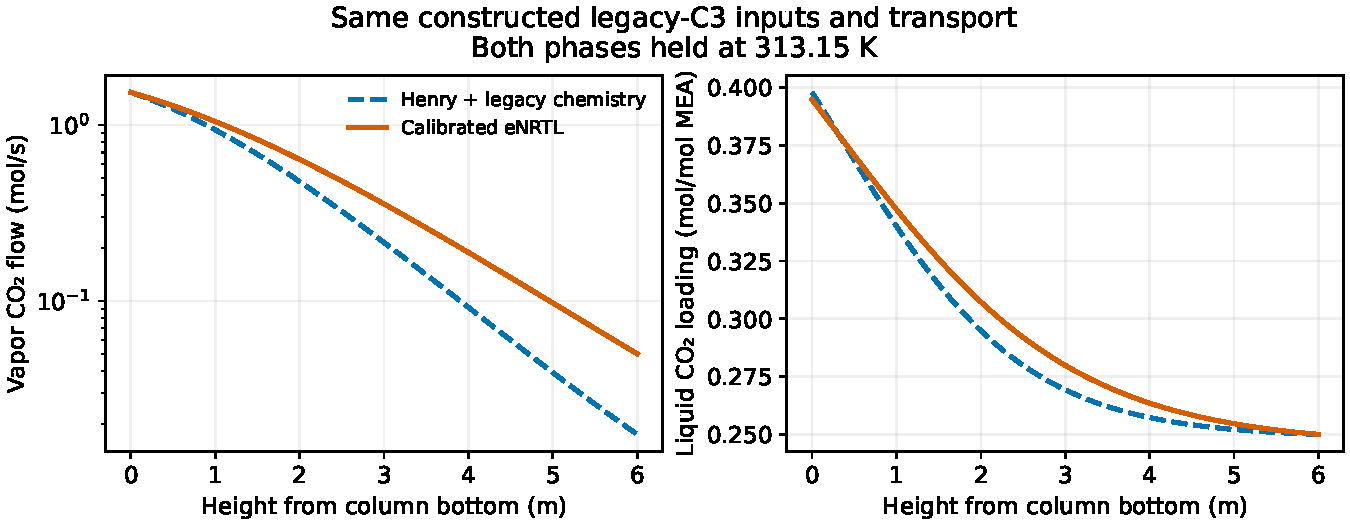
\includegraphics[width=\linewidth]{figures/isothermal-henry-enrtl-profiles.pdf}
% P:results-isothermal-caption
\caption{Calculated vapor CO$_2$ flow and apparent liquid loading for the constructed C3 isothermal control at \qty{313.15}{K}.
The Henry-law reference retains its conventional reaction description, whereas the eNRTL arm uses the calibrated six-species model; both use the same feeds and conventional transport.
The vapor-flow axis is logarithmic, and height increases from the gas inlet.
Profiles use the solutions initialized with 33 axial points.}
\label{fig:isothermal-control}
\end{figure}

\subsubsection{Density and caloric effects}
% P:results-10
\Cref{fig:full-property} extends the equilibrium comparison to the consistent density and enthalpy response of the selected thermodynamic description.
For any reported quantity $Q$, the paired changes can be written
\begin{align}
\Delta Q_{\mathrm{eq}}&=Q_{\mathrm{common},m}-Q_{\mathrm{common},\mathrm{ref}},\\
\Delta Q_{\mathrm{prop}}&=Q_{\mathrm{full},m}-Q_{\mathrm{common},m}.
\end{align}
Here $m$ denotes the thermodynamic model and the reference denotes the common-property comparison basis.
These paired changes follow the specified sequence of model substitutions.
They distinguish the equilibrium comparison from its additional volume and energy response, conditional on the retained transport model; a different substitution order can assign interacting effects differently.

% CHECKLIST-BEGIN: finding-3
% P:results-11
\noindent\textit{[Quantitative comparison: additional capture change, temperature-maximum change and axial shift, and temperature-tap RMSE for the full-property calculation.]}
% CHECKLIST-END: finding-3

% P:results-12
Density changes affect volumetric flow, velocity, holdup, and transfer coefficients.
Caloric changes alter the temperature response to the same local absorption and water transfer.
Because temperature feeds back into equilibrium and mobility, the full-property effect is interpreted through the coupled profiles rather than by adding isolated property errors.
The paired simulations retain the same feeds and packing specification throughout this comparison.

\begin{figure}[pos=htbp]
\centering
\fbox{\begin{minipage}[c][55mm][c]{0.93\linewidth}\centering
\textbf{Equilibrium and full-property effects}\\[8mm]
\small (a) Paired changes in capture\\[3mm](b) Liquid temperature and volumetric flow\\[3mm](c) Enthalpy and absorption distribution
\end{minipage}}
% P:results-13
\caption{Comparison of common-property and full-property calculations at matched operating conditions.
The panels separate the initial equilibrium/fugacity change from the additional density and caloric response.}
\label{fig:full-property}
\end{figure}
% Replace the framed panel with the final figure; keep this label and update the caption to its exact case set.

\subsection{Thermodynamic parameter sensitivity}\label{subsec:results-sensitivity}
% P:results-sensitivity-01
The preceding model comparison changes the thermodynamic description; the sensitivity comparison varies four parameter coordinates within the selected ePC-SAFT description at the Case 3C reference conditions.
The perturbation definitions are given in \cref{subsec:sensitivity-design}.
\Cref{fig:thermodynamic-sensitivity} distinguishes the locally recomputed driving force from the response after the complete column is resolved.
The local comparison retains analytical flows and temperature, while the coupled comparison allows absorption and heat release to redistribute along the bed.
A change in local fugacity therefore need not produce a proportional change in capture.

% CHECKLIST-BEGIN: finding-10
% P:results-sensitivity-02
\textit{[Thermodynamic sensitivity: signed capture and temperature changes for each prescribed perturbation, local and coupled fugacity/flux responses, and their size relative to numerical refinement.]}
% CHECKLIST-END: finding-10

\begin{figure}[pos=htbp]
\centering
\fbox{\begin{minipage}[c][48mm][c]{0.93\linewidth}\centering
\textbf{Case 3C thermodynamic sensitivity}\\[8mm]
\small (a) Signed capture and temperature changes\\[3mm](b) Local and coupled driving-force response
\end{minipage}}
\caption{Response to the two reaction-enthalpy directions, water solvation factor, and CO$_2$ dispersion energy at the Case 3C reference inputs. The positive and negative perturbations use the ranges in \cref{tab:operating-sensitivity-inputs}; capture changes are in percentage points and temperature changes in kelvin.}
\label{fig:thermodynamic-sensitivity}
\end{figure}

\subsection{Enhancement-factor and reactive-film transport}\label{subsec:results-film}
% P:results-film-transition
The thermodynamic comparisons describe the availability of CO$_2$ for transfer.
The film comparison examines how the liquid resistance converts that driving force into uptake at the same thermodynamic model and feed conditions.
\subsubsection{Capture and local transfer resistance}
% P:results-14
\Cref{fig:film-capture} compares the enhancement-factor and equilibrium-manifold transfer descriptions at common bulk thermodynamics.
The model difference is the representation of liquid-film resistance.
Both arms retain the same feed definitions, reaction equilibrium, gas-side resistance, water transfer, and packing correlations.
Their axial bulk states are independently calculated consequences of the selected film model.
The signed transfer-model effect for case $k$ is
\begin{align}
\Delta\eta_{k,\mathrm{film}}=\eta_{k,\mathrm{film}}-\eta_{k,\mathrm{enh}}.
\end{align}

% CHECKLIST-BEGIN: finding-4
% P:results-15
\noindent\textit{[Quantitative comparison: the range of capture changes, aggregate capture errors, and operating conditions associated with the largest transfer-model effect.]}
% CHECKLIST-END: finding-4

% P:results-16
The local interpretation follows the interfacial state and the integrated liquid resistance.
In the enhancement description, the Hatta number and finite reactant supply determine the effective liquid-film contribution.
In the equilibrium-manifold description, the reactive chemical-potential tangent and constrained mobility determine that contribution along the complete bulk-to-interface path.
These representations can be compared through their resulting fluxes without assigning the film calculation an empirical enhancement multiplier.

\begin{figure}[pos=htbp]
\centering
\fbox{\begin{minipage}[c][55mm][c]{0.93\linewidth}\centering
\textbf{Transfer-model comparison}\\[8mm]
\small (a) Enhancement and reactive-film capture\\[3mm](b) Casewise capture change\\[3mm](c) Local gas- and liquid-film resistance
\end{minipage}}
% P:results-17
\caption{Enhancement-factor and equilibrium-manifold film comparisons with the same thermodynamic model and feed conditions.
Each arm solves its own axial bulk states.
Positive capture change denotes greater uptake for the equilibrium-manifold calculation.}
\label{fig:film-capture}
\end{figure}
% Replace the framed panel with the final figure; keep this label and update the caption to its exact case set.

\subsubsection{Interfacial state and axial absorption}
% P:results-18
\Cref{fig:film-profiles} follows the local CO$_2$ flux, interfacial fugacity, and cumulative uptake along the bed.
The interface-root solution partitions the total driving force between gas and liquid resistances.
This partition connects a change in the local film law to the axial region in which the column response changes.
The cumulative uptake in \cref{eq:integral-uptake} then relates the local comparison to the total capture.

% CHECKLIST-BEGIN: finding-5
% P:results-19
\noindent\textit{[Principal finding: the dominant resistance, the axial region of the largest flux change, and the resulting redistribution of cumulative uptake.]}
% CHECKLIST-END: finding-5

% P:results-20
The film comparison also distinguishes a higher total uptake from a different distribution of uptake.
Two calculations can have similar outlet capture while locating absorption and heat release differently within the bed.
The interfacial and temperature profiles are therefore interpreted together with the integrated performance.
The water-transfer contribution is retained in the energy balance even though the CO$_2$ mobility calculation constrains its own water-component flux.

\begin{figure}[pos=htbp]
\centering
\fbox{\begin{minipage}[c][55mm][c]{0.93\linewidth}\centering
\textbf{Transfer-model comparison: axial response}\\[8mm]
\small (a) CO$_2$ flux and interfacial fugacity\\[3mm](b) Cumulative absorbed CO$_2$\\[3mm](c) Liquid and gas temperature
\end{minipage}}
% P:results-21
\caption{Axial transfer and temperature profiles for the enhancement-factor and equilibrium-manifold calculations.
Local fluxes integrate to the inlet/outlet material balance; cumulative uptake distinguishes total capture from its spatial distribution.}
\label{fig:film-profiles}
\end{figure}
% Replace the framed panel with the final figure; keep this label and update the caption to its exact case set.

\subsubsection{Mobility and film-thickness sensitivity}
% P:results-film-sensitivity-intro
\Cref{fig:film-sensitivity} relates changes in capture and temperature to species-group mobility and film thickness.
The separate perturbations defined in \cref{subsec:film-sensitivity-design} identify which transport inputs most influence the comparison with the enhancement-factor model.

% CHECKLIST-BEGIN: finding-6
% P:results-24
\noindent\textit{[Sensitivity findings: the influential mobility inputs, the selected perturbation ranges, the capture and temperature changes, and the persistence of the transfer-model comparison over those ranges.]}
% CHECKLIST-END: finding-6

% P:results-25
The mobility approximation represents species transport, while the equilibrium tangent represents thermodynamic response.
Keeping these contributions separate identifies whether a model difference is controlled mainly by the reaction-equilibrium path or by the assumed transport scale.
The sensitivity range follows the parameter sources and the stated physical assumptions, rather than a fit to the column capture observations.

\begin{figure}[pos=htbp]
\centering
\fbox{\begin{minipage}[c][48mm][c]{0.93\linewidth}\centering
\textbf{Film-input sensitivity}\\[8mm]
\small (a) Capture response to diffusivity groups\\[3mm](b) Capture and temperature response to film thickness
\end{minipage}}
% P:results-26
\caption{Sensitivity of the equilibrium-manifold calculation to the specified species diffusivities and physical film thickness.
Thermodynamic parameters and case inputs are held fixed.}
\label{fig:film-sensitivity}
\end{figure}
% Replace the framed panel with the final figure; keep this label and update the caption to its exact case set.

\subsection{Boundary-value solution methods}\label{subsec:results-solvers}
\subsubsection{Solution agreement and refinement}
% P:results-27
\Cref{fig:solver-accuracy} compares the conservative simultaneous formulation with shooting, finite differences, and collocation on identical physical equations.
The comparison uses capture, liquid-temperature profiles, and the integral balances to relate the numerical solutions.
Refinement varies the axial resolution and film quadrature separately, preserving the physical inputs.
The profile comparison includes the temperature maximum and its location, which can be more sensitive to resolution than the integrated capture.

% CHECKLIST-BEGIN: numerical-node-verification
% P:results-node-verification
A local verification of the conservative formulation compares the assembled $19\times12$ Jacobian with a centered directional difference at a synthetic interior test state, using a step of $10^{-3}$ along the prescribed physical direction.
The maximum rowwise relative discrepancy is $2.05\times10^{-7}$; the liquid-film, gas-CO$_2$, water-transfer, and energy rows give $6.22\times10^{-9}$, $7.70\times10^{-9}$, $2.83\times10^{-9}$, and $1.89\times10^{-10}$, respectively.
Each discrepancy is scaled by the larger magnitude of the analytic and difference estimates, with a denominator floor of $10^{-12}$.
The test-state construction and implementation identity are supplied in the supplementary verification record.
This comparison verifies derivative assembly at the tested state; full-column solution agreement and refinement are assessed separately in \cref{fig:solver-accuracy}.
% CHECKLIST-END: numerical-node-verification

% CHECKLIST-BEGIN: finding-7
% P:results-28
\noindent\textit{[Numerical findings: agreement in capture and temperature, mesh and quadrature refinement changes, and material/energy/charge conservation at the reported settings.]}
% CHECKLIST-END: finding-7

% P:results-29
The methods represent the same countercurrent coupling differently.
Shooting resolves it through a boundary root around an initial-value integration; finite differences solve a nodal algebraic system; collocation uses a continuous polynomial representation with residual-based refinement; the conservative simultaneous formulation balances physical flow quantities directly between nodes.
The comparison therefore associates cost with a specified solution accuracy and operating point.
It does not combine different physical models in a numerical-method ranking.

\begin{figure}[pos=htbp]
\centering
\fbox{\begin{minipage}[c][55mm][c]{0.93\linewidth}\centering
\textbf{Boundary-value solution accuracy}\\[8mm]
\small (a) Cross-method axial profiles\\[3mm](b) Capture and temperature changes with refinement\\[3mm](c) Integral material and energy balance
\end{minipage}}
% P:results-30
\caption{Solution agreement and refinement for conservative simultaneous, shooting, finite-difference, and collocation formulations applied to the same absorber equations.
Profile comparisons use common physical heights and the same inlet specification.}
\label{fig:solver-accuracy}
\end{figure}
% Replace the framed panel with the final figure; keep this label and update the caption to its exact case set.

% CHECKLIST-BEGIN: method-09
% P:methods-21
\Cref{tab:numerical-comparison} reports the accuracy and cost of each method at the same operating point and with the same physical equations.
Refinement changes are differences from the next finer calculation, while conservation errors are evaluated from the dimensional balances.

\begin{table}[pos=htbp]
\centering\small
\caption{Boundary-value method comparison at matched physical conditions. Capture refinement changes are in percentage points, temperature changes in kelvin, and runtime in seconds. The conservation column reports the scaled material, energy, and charge residuals.}
\label{tab:numerical-comparison}
\begin{tabularx}{\linewidth}{@{}lXXXXX@{}}
\toprule
Method & Nodes & $|\Delta\eta|$ & $\|\Delta T_l\|_\infty$ & Conservation & Runtime\\
\midrule
Shooting & \textit{[value]} & \textit{[value]} & \textit{[value]} & \textit{[values]} & \textit{[values]}\\
Finite differences & \textit{[value]} & \textit{[value]} & \textit{[value]} & \textit{[values]} & \textit{[values]}\\
Collocation & \textit{[value]} & \textit{[value]} & \textit{[value]} & \textit{[values]} & \textit{[values]}\\
Conservative simultaneous & \textit{[value]} & \textit{[value]} & \textit{[value]} & \textit{[values]} & \textit{[values]}\\
\bottomrule
\end{tabularx}
\end{table}
% CHECKLIST-END: method-09

\subsubsection{Computational cost}
% P:results-31
\Cref{fig:solver-cost} relates runtime to the achieved accuracy and identifies the contribution of local thermodynamics and film evaluation.
Repeated timings use the same hardware, thread configuration, and scope of calculation.
The timing comparison distinguishes a change in the number of local evaluations from a change in their individual cost.

% CHECKLIST-BEGIN: finding-8
% P:results-32
\noindent\textit{[Timing findings: median runtime and spread for each method, evaluation counts, final mesh sizes, and the operating-point dependence of the preferred method.]}
% CHECKLIST-END: finding-8

% P:results-33
A more expensive local thermodynamic model can change the balance between integration work and global nonlinear iterations.
The cost of the reactive film also depends on the quadrature resolution required along the equilibrium path.
The comparison is therefore interpreted jointly with the refinement results: the relevant computational saving is the reduction in time to obtain the same physical quantities to the same accuracy.

\begin{figure}[pos=htbp]
\centering
\fbox{\begin{minipage}[c][48mm][c]{0.93\linewidth}\centering
\textbf{Boundary-value solution cost}\\[8mm]
\small (a) Runtime versus achieved accuracy\\[3mm](b) Equilibrium, film, and column-solve contributions
\end{minipage}}
% P:results-34
\caption{Computational cost of the BVP formulations at matched numerical accuracy.
Timing scope, repeated-run summary, hardware, and thread configuration accompany the final comparison.}
\label{fig:solver-cost}
\end{figure}
% Replace the framed panel with the final figure; keep this label and update the caption to its exact case set.

\subsection{Operating-condition response}\label{subsec:results-operating}
% P:results-operating-01
\Cref{fig:operating-screen} relates the sampled operating conditions to capture, gas and liquid outlet temperatures, and the temperature maxima and their locations.
Gas throughput and liquid circulation are described on the mass basis defined in \cref{subsec:sensitivity-design}, while lean loading and MEA fraction determine the incoming solvent composition.
The thermodynamic and transport coordinates vary alongside these operating inputs, so response trends are interpreted jointly rather than assigned to a single operating variable from an unadjusted scatter plot.
The common diffusivity multiplier examines the overall mobility scale; it does not resolve relative uncertainty among individual ionic diffusivities.

% CHECKLIST-BEGIN: finding-11
% P:results-operating-02
\textit{[Operating-condition findings: sampled capture and temperature ranges, supported response directions and input rankings, additive-model prediction quality, and the operating tradeoffs supported within the sampled domain.]}
% CHECKLIST-END: finding-11

% P:results-operating-03
The operating comparison extends the reference-case sensitivity in \cref{subsec:results-sensitivity} to simultaneous changes in feeds, thermodynamic parameters, and transport properties.
Capture and the thermal response are considered jointly within the selected ranges.
Their comparison is conditional on the one-bed geometry, assumed inlet humidity and liquid temperature, and fixed gas temperature and pressure specification.
An operating point with higher capture may require greater solvent circulation or alter the temperature maximum; those consequences are retained in the comparison.
A plant-level optimum additionally depends on regeneration duty, hydraulic limits, and the selected economic or energy objective.

\begin{figure}[pos=htbp]
\centering
\fbox{\begin{minipage}[c][48mm][c]{0.93\linewidth}\centering
\textbf{Local operating-condition comparison}\\[8mm]
\small (a) Capture and thermal response across sampled conditions\\[3mm](b) Supported thermodynamic, transport, and operating effects
\end{minipage}}
\caption{Capture and temperature response for the 48-point Latin hypercube design around Case 3C. The input ranges are given in \cref{tab:operating-sensitivity-inputs}; the response panels use the sampled operating conditions, and the ranges are exploratory rather than probability intervals.}
\label{fig:operating-screen}
\end{figure}

\subsection{Integrated absorber response and engineering interpretation}\label{subsec:results-implications}
% P:results-35
The model comparisons and sensitivity studies connect the representation of the absorber to its operating response.
The thermodynamic comparison identifies the effect of equilibrium and property descriptions, while the parameter study identifies the inputs that control that response within ePC-SAFT.
The film comparison isolates the transfer treatment at common thermodynamics, and the numerical comparison quantifies the effort needed to resolve the same physical equations.
The Latin hypercube study examines how these dependencies influence capture and temperature over the specified operating neighborhood.

% CHECKLIST-BEGIN: finding-9
% P:results-36
\noindent\textit{[Cross-study synthesis: relative magnitude of thermodynamic, transfer, and numerical effects; the supported choice of model and solution method; the sensitivity and operating tradeoffs that qualify that choice; the capture and temperature evidence supporting the interpretation.]}
% CHECKLIST-END: finding-9

% P:results-37
The experimental temperature profile provides a spatial constraint on this interpretation.
Agreement in capture is accompanied by the position and magnitude of heat release, with water evaporation and interphase heat exchange represented in the same energy balance.
A comparison that improves one observable is assessed against its effect on the others.
The physical assumptions remain the local reaction-equilibrium approximation, the mobility description, nontransfer of MEA and gas inerts, the separate water-transfer law, and the parameter temperature domains.

% P:results-38
The scope is a one-bed absorber with specified feeds and packing.
Extensions to intercooling, substantial pressure drop, or additional volatile components require the corresponding material and energy terms.
The results of the controlled studies provide the basis for selecting which thermodynamic and transfer detail is needed for the operating range examined here.


    \section{Conclusions}\label{sec:conclusions}
% P:conclusion-01
The absorber formulation connects reactive ePC-SAFT thermodynamics to a constrained equilibrium-manifold film and countercurrent material and energy balances.
The local film resistance is obtained by quadrature in reactive state space and a scalar interface balance, while the axial column remains a two-point boundary-value problem.
Consistent species amounts, conserved totals, and enthalpy references connect equilibrium, transport, and the thermal response.

% P:conclusion-02
The comparisons relate thermodynamic model choice, parameter sensitivity, film resistance, and computational effort to the same capture and temperature observables.
The local operating study places those dependencies within a specified range of feeds and property inputs.
% INSERT final quantitative conclusions for thermodynamics and parameter sensitivity, transfer, solution cost, and operating response, in that order.
% INSERT the engineering implication supported jointly by capture and axial-temperature comparisons.

% P:conclusion-03
The thermodynamic study connects the Henry-law, eNRTL, and ePC-SAFT driving-force descriptions to capture and axial temperature.
The common-property comparison identifies the response to the selected thermodynamic description, including its specified species and reaction system.
The full-property comparison identifies the additional density and caloric response under the same transport assumptions.
The parameter sensitivity then distinguishes the influence of reaction-enthalpy directions, water solvation, and CO$_2$ dispersion within the selected ePC-SAFT description.
% CHECKLIST-BEGIN: conclusion-1
% P:conclusion-04
\textit{[Insert the principal thermodynamic finding, its quantitative effect, and the parameter-sensitivity finding that qualifies it.]}
% CHECKLIST-END: conclusion-1

% P:conclusion-05
The transfer study compares the enhancement-factor and equilibrium-manifold resistance with the same thermodynamic model and feed conditions.
The interfacial state, flux distribution, and cumulative uptake explain the resulting column response.
% CHECKLIST-BEGIN: conclusion-2
% P:conclusion-06
\textit{[Insert the principal transfer finding, capture effect, and mobility-sensitivity conclusion.]}
% CHECKLIST-END: conclusion-2

% P:conclusion-07
The numerical study compares conservative simultaneous, shooting, finite-difference, and collocation formulations at common physical conditions and solution accuracy.
% CHECKLIST-BEGIN: conclusion-3
% P:conclusion-08
\textit{[Insert the method comparison, runtime effect, and refinement-supported accuracy.]}
% CHECKLIST-END: conclusion-3

% P:conclusion-synthesis
Together, the three studies relate absorber performance to the selected thermodynamic model, the local film representation, and the numerical work needed to resolve the coupled balances.
The operating comparison extends that interpretation to the specified neighborhood around Case 3C.
% CHECKLIST-BEGIN: conclusion-4
% P:conclusion-operating-finding
\textit{[Insert the supported operating tradeoff and the combined capture/temperature implication for model selection.]}
% CHECKLIST-END: conclusion-4


\subsection{Applicability and future work}\label{subsec:applicability}
% P:conclusion-09
The formulation applies to a steady, one-bed MEA absorber within the composition, temperature, and pressure domains of its thermodynamic and transport inputs.
Parameter uncertainty and extrapolation beyond the source ranges can affect speciation, transfer, and heat release together.
The equilibrium-manifold film assumes rapid local reaction and an isothermal diffusion path; conditions in which reaction or thermal relaxation competes with diffusion require finite-rate species and energy balances in the film.
Industrial gas mixtures containing additional reactive or volatile components require their species, reactions, properties, and interphase transfer terms.

% P:conclusion-10
The column balances and numerical formulations can be reused for DEA, MDEA, AMP, PZ, or blended solvents after defining the solvent-specific chemistry and constitutive inputs.
The extension begins with a reaction network, conserved components, and consistent activity and enthalpy reference states.
Pure-component, binary, association, ionic, and dielectric parameters are obtained from applicable sources or fitted to independent thermodynamic measurements, including VLE, speciation, and caloric data where available.
Transport properties and kinetic parameters are then specified for the solvent and packing.
Thermodynamic measurements excluded from fitting and independent absorber measurements evaluate the parameterization and the coupled column model, respectively.
A parameter-file substitution alone does not establish transferability to another solvent.

% P:conclusion-11
The specified input ranges of the Latin hypercube design define the domain of the operating comparison; they do not establish a global operating optimum.
Formal optimization additionally requires a stated objective and hydraulic, thermal, and process constraints.
Coupling the absorber to solvent regeneration would permit energy or economic objectives beyond capture alone.
These extensions should preserve the separation between property fitting, numerical verification, and experimental evaluation.


    \appendix

    \section{Property Definitions and Parameter Reporting}\label{sec:properties}
\subsection{Species and amount bases}
% P:appendix-properties-01
\Cref{tab:species-basis} distinguishes apparent components from the true species used in equilibrium and transport.
The material, mass, and charge constraints in \cref{eq:conserved-totals,eq:complete-invariants} fix the conversion between these representations.
Molar density and enthalpy are evaluated on the true-species amount basis before conversion to column flow quantities.

\begin{table}[pos=htbp]
\centering\small
\caption{Component and species definitions in the absorber formulation.}
\label{tab:species-basis}
\begin{tabularx}{\linewidth}{@{}p{0.24\linewidth}X@{}}
\toprule
Representation & Components or species\\
\midrule
Apparent liquid & CO$_2$, MEA, H$_2$O\\
True liquid & CO$_2$, MEA, H$_2$O, MEAH$^+$, MEACOO$^-$, HCO$_3^-$, CO$_3^{2-}$, H$_3$O$^+$, OH$^-$\\
Gas & CO$_2$, H$_2$O, N$_2$, O$_2$\\
Interphase transfer & CO$_2$ and H$_2$O\\
Nontransferring components & MEA in the liquid; N$_2$ and O$_2$ in the gas\\
\bottomrule
\end{tabularx}
\end{table}

\subsection{Equilibrium and reference properties}\label{sec:appendix-properties}
% P:appendix-properties-02
Reaction constants are dimensionless and paired with their stated activity conventions.
Temperature correlations retain the coefficient units, logarithm base, and temperature domain of their source representation.
The reference enthalpy and heat-capacity conventions are common to the equilibrium and caloric calculations.
Species identity and order are the same in the reaction system, thermodynamic parameters, reference properties, and film mobility.
% CHECKLIST-BEGIN: method-11
% P:appendix-properties-03
The coefficients in \cref{tab:reactive-constants} use the aqueous infinite-dilution molality convention with water solvent, $m^\circ=\qty{1}{mol\,kg^{-1}}$, and $P^\circ=\qty{1}{bar}$.
For R1--R3 the additional linear-in-temperature coefficient is zero.
R1 and R3 retain additive standard-state shifts $2s$ and $s$, respectively, with $s=4.0165349923$.
The fitted R2 coefficient $a_2$ already includes this conversion, so its additional offset is zero.
The selected R2, R4, and R5 temperature correlations replace their source correlations as complete coefficient sets.

\begin{table}[pos=htbp]
\centering
\caption{Reaction-constant coefficients for \cref{eq:reaction-constants}. Temperature is evaluated in kelvin. R1--R3 include the standard-state offsets; R4 and R5 use their distinct forms.}
\label{tab:reactive-constants}
\small
\begin{tabular}{@{}lrrrr@{}}
\toprule
Reaction & $a_r$ & $b_r$ & $c_r$ & $s_r$ \\
\midrule
R1 & 132.899 & $-13445.9$ & $-22.4773$ & 8.0330699846 \\
R2 & 232.331415338844 & $-11105.6400305203$ & $-36.7816$ & 0 \\
R3 & 216.049 & $-12431.7$ & $-35.4819$ & 4.0165349923 \\
\midrule
R4 & \multicolumn{4}{l}{$a_4=1.505015374192114$, $b_4=-1317.0489707842564$} \\
R5 & \multicolumn{4}{l}{$A_5=3037.6399534696106$, $B_5=-1.0173150837285996$, $C_5=0.0004277$} \\
\bottomrule
\end{tabular}
\end{table}

\begin{table}[pos=htbp]
\centering\small
\caption{Temperature intervals assigned to the reaction correlations. A model evaluation interval does not enlarge the underlying source interval.}
\label{tab:reaction-temperature-intervals}
\begin{tabular}{@{}ll@{}}
\toprule
Reaction & Evaluation interval (K)\\
\midrule
R1, R3 & 273.15--498.15\\
R2, R4 & 293.15--393.15\\
R5 & 293.15--393.15\\
\bottomrule
\end{tabular}
\end{table}

% P:appendix-properties-04
The underlying source intervals are \qtyrange{273.15}{498.15}{K} for the R1--R3 forms, \qtyrange{293.15}{323.15}{K} for R4, and \qtyrange{273.15}{323.15}{K} for R5.
Use of R4 or R5 above \qty{323.15}{K} extrapolates the respective source relation.
% CHECKLIST-REVIEW: Typed fitted R2/R4/R5 from parameter a9186c93 replace complete source correlations; no second R2 offset. Retain primary-source/domain review and match the final run identity; see SOURCE_MAP.md.

% CHECKLIST-END: method-11
% CHECKLIST-BEGIN: method-10
% P:appendix-properties-05
The ePC-SAFT description uses the nine pure-component records in \cref{tab:reactive-pure-parameters}, general-site association, Debye--H\"uckel electrostatics, the original Born contribution, and solvent-only MEA/water relative-permittivity mixing.
For the dispersion combining rule,
\begin{align}
\epsilon_{ij}=\sqrt{\epsilon_i\epsilon_j}(1-k_{ij}),\qquad k_{ij}=k_{ji}.
\end{align}
All like-charge ionic pairs have $k_{ij}=1$ and therefore zero unlike-pair dispersion energy.
All other distinct pairs have $k_{ij}=0$ except those listed in \cref{tab:reactive-pair-parameters}; together these rules specify all 36 distinct pairs.
The CO$_2$/MEA reciprocal-temperature slope is zero.

\begin{table}[pos=htbp]
\centering\small
\caption{Nonzero dispersion corrections outside the like-charge rule. Values are dimensionless and symmetric in species indices.}
\label{tab:reactive-pair-parameters}
\begin{tabularx}{\linewidth}{@{}lrX@{}}
\toprule
Pair & $k_{ij}$ & Parameter treatment\\
\midrule
\ce{CO2}/\ce{H2O} & 0.0132628791769 & Fixed mixture correction\\
\ce{MEA}/\ce{H2O} & $-0.0735274987499$ & Fitted to neutral MEA/water VLE\\
\ce{MEAH+}/\ce{MEACOO-} & $-0.00201813457644$ & Fixed historical electrolyte value\\
\ce{CO3^2-}/\ce{H2O} & $-0.25$ & Assigned ion/water correction\\
\ce{H3O+}/\ce{H2O} & 0.25 & Assigned ion/water correction\\
\ce{OH-}/\ce{H2O} & $-0.25$ & Assigned ion/water correction\\
\bottomrule
\end{tabularx}
\end{table}

% P:appendix-parameter-origin
The MEA/water binary correction is fitted to a 25-point neutral-mixture VLE dataset using pressure-level groups for model selection and a final fit to the complete dataset.
The other nonzero pair values in \cref{tab:reactive-pair-parameters} are fixed inputs: the molecular CO$_2$/water correction and ion/water corrections are specified mixture assumptions, and the MEAH$^+$/MEACOO$^-$ correction is retained from the starting electrolyte parameterization.
Like-charge dispersion exclusion follows the selected combining rule \cite{Figiel2025}.
These distinct origins separate parameter estimation from the physical assumptions used in the column calculation.

% P:appendix-parameter-fit
The CO$_2$ dispersion energy is selected against pressure and speciation measurements, while the remaining pure-component segment and ionic diameter values are adopted from the starting parameterization.
The R2, R4, and R5 temperature coefficients are adjusted through reaction-enthalpy shifts while preserving their equilibrium constants at \qty{313.15}{K}.
The reaction-temperature fit uses pressure and speciation targets together with six calorimetric intervals from Kim and Svendsen \cite{Kim2007}; its pressure targets include Jou et al. measurements at \qty{393.15}{K} \cite{Jou1995}.
The Xu pressure measurements and the calorimetry block at \qty{393.15}{K} are excluded from the fitting objective and used for separate thermodynamic evaluation \cite{Xu2011,Kim2007}, while the Kim et al. measurements provide a model-selection comparison \cite{Kim2014}.
The resulting reaction functions and the neutral caloric anchors jointly determine the ionic reference enthalpies and heat capacities.
Absorber capture and temperature profiles provide a separate column evaluation rather than the targets of these property fits.
% CHECKLIST-REVIEW: Parameter a9186c93 source IDs cai-1996-neutral-refit, mea-best-in-slot-campaign-2026-09-02, and mea-reaction-temperature-fit-2026-09-03 identify these fits. Preserve upstream fit/source files and complete primary bibliography locators in the final data deposit.

% P:appendix-properties-06
MEA, water, and CO$_2$ each have one donor-labelled site $a$ and one acceptor-labelled site $b$ in the selected topology.
The explicit association pairs are reported in \cref{tab:reactive-association}; site labels denote the model topology, including induced association of CO$_2$.
The two MEA/water cross pairs use arithmetic averaging of association energies and geometric averaging of association volumes.
No other site pairs are active, and the ionic species have no association sites in this parameterization.

\begin{table}[pos=htbp]
\centering\small
\caption{Explicit association parameters. MEA/water cross association uses the combining rules stated in the text.}
\label{tab:reactive-association}
\begin{tabular}{@{}lrr@{}}
\toprule
Site pair & $\epsilon^{AB}/k$ (K) & $\kappa^{AB}$\\
\midrule
MEA $a$ / MEA $b$ & 2586.3 & 0.03747\\
Water $a$ / water $b$ & 2425.7 & 0.04509\\
CO$_2$ $a$ / water $b$ & 1212.85 & 0.04509\\
CO$_2$ $b$ / water $a$ & 1212.85 & 0.04509\\
\bottomrule
\end{tabular}
\end{table}

% P:appendix-properties-07
The MEA relative permittivity is 32, and the ionic-region value is 8.
For water, with $\Delta T=T-298.15\,\mathrm K$ evaluated numerically in kelvin,
\begin{align}
\varepsilon_{r,W}=78.4104347858-0.361337662337\Delta T
+0.00076555618295(\Delta T)^2.
\end{align}
The salt-free solvent relative permittivity uses mass fractions normalized over the neutral MEA and water solvent species \cite{Figiel2025}:
\begin{align}
w_i^{\mathrm{solv}}&=\frac{n_iM_i}{n_A M_A+n_W M_W},\qquad i\in\{A,W\},\\
\varepsilon_r(T,\mathbf n)&=32w_A^{\mathrm{solv}}+\varepsilon_{r,W}(T)w_W^{\mathrm{solv}}.
\label{eq:solvent-permittivity}
\end{align}
Here $n_A$ is the amount of neutral MEA, rather than the total apparent amine amount.
CO$_2$ and ionic species are excluded from this solvent normalization.
The common parameter-evaluation interval is \qtyrange{293.15}{393.15}{K}; the individual reaction-source intervals are distinguished in \cref{tab:reaction-temperature-intervals}.
% CHECKLIST-REMAINING: Add the selected eNRTL pure/pair and model-specific reference records. The ePC-SAFT coefficient treatment and solvent-only dielectric equation are documented; complete primary-source locators and match final run identities in SOURCE_MAP.md.

\begin{table}[pos=htbp]
\centering\small
\caption{Additional thermodynamic inputs for the activity-coefficient comparison and solvent dielectric mixing. The ePC-SAFT pair and association coefficients are given in the preceding tables.}
\label{tab:comparison-thermo-inputs}
\begin{tabularx}{\linewidth}{@{}lX@{}}
\toprule
Input & Definition and coefficients\\
\midrule
eNRTL species and reactions & CO$_2$, MEA, H$_2$O, MEAH$^+$, MEACOO$^-$, HCO$_3^-$; the two formation reactions in \cref{eq:enrtl-combined-reactions}\\
eNRTL interactions & \textit{[Molecule/molecule, molecule/ion-pair, and ion-pair records]}\\
eNRTL temperature dependence & \textit{[Interaction forms, nonrandomness, and coefficient units]}\\
Solvent dielectric mixing & Neutral-solvent mass fractions; \cref{eq:solvent-permittivity}\\
eNRTL reference conversion & \textit{[Model-specific solute reference offsets]}\\
eNRTL parameter sources & \textit{[Source records and applicable domains]}\\
\bottomrule
\end{tabularx}
\end{table}

% CHECKLIST-END: method-10
% INSERT Table: reference enthalpies/heat capacities, units and amount basis, standard pressure, temperature ranges, sources, and the fixed-P/conserved-total equilibrium derivative convention.
% Preserve any source-domain extrapolation explicitly alongside the affected parameter; do not hide it in workflow prose.

\subsection{Transport and packing correlations}
% P:appendix-properties-08
The Henry-law reference uses a concentration-based coefficient consistent with \cref{eq:henry}; the N$_2$O analogy provides the solvent-mixture solubility relation \cite{Jiru2012}.
Viscosity, surface tension, and diffusivity correlations supply the physical transport properties \cite{Morgan2015}.
Packing area, void fraction, hydraulic diameter, and correlation coefficients define the hydraulic model \cite{Billet1999,Tsai2010,Chinen2018}.
Within each controlled comparison, these inputs remain common except for the property group explicitly varied in \cref{tab:comparison-design}.

% P:appendix-properties-09
The mobility diffusivities $D_i$ describe individual true species, whereas $D_C^{\mathrm{column}}$ defines the physical film thickness in \cref{eq:film-thickness}.
The distinction preserves the respective meanings of the mobility approximation and the packed-column mass-transfer correlation.
% CHECKLIST-BEGIN: method-13
% P:appendix-properties-10
The coefficient tables below define the common-property calculation on an apparent liquid-component basis and a four-component gas basis.
Temperature is in kelvin unless a Celsius variable is explicitly defined, and empirical coefficients absorb the units needed by their stated expressions.
The selected holdup relation is
\begin{align}
h_l^*&=11.4474\left[3.185966\,u_l(\mu_l/\rho_{l,m})^{1/3}\right]^{0.6471},\\
h_l&=\frac{\varepsilon h_l^*}{\varepsilon+h_l^*},\qquad h_v=\varepsilon-h_l,
\label{eq:common-holdup}
\end{align}
using $u_l$ in \unit{m\,s^{-1}}, $\mu_l$ in \unit{Pa\,s}, and $\rho_{l,m}$ in \unit{kg\,m^{-3}}.
The rational mapping keeps the liquid holdup below the packing void fraction.
For gas component $j$, the fugacity-based transfer coefficient and the heat-transfer analogy are
\begin{align}
k_{g,j}&=\frac{C_V}{RT_v}\sqrt{\frac{a_p}{d_hh_v}}D_{v,j}^{2/3}
\left(\frac{\mu_v}{\rho_{v,m}}\right)^{1/3}
\left(\frac{u_v\rho_{v,m}}{a_p\mu_v}\right)^{3/4},\\
U_T&=\left[\frac{(k_{g,C}P)^3 k_{t,v}^{\,2}c_{p,v}}
{(\rho_vD_{v,C})^2}\right]^{1/3}.
\label{eq:common-gas-heat-transfer}
\end{align}
Here $\rho_v$ is gas molar density, $\rho_{v,m}$ is gas mass density, $c_{p,v}$ is molar heat capacity, and $k_{t,v}$ is gas thermal conductivity.
The resulting units are \unit{mol\,m^{-2}\,s^{-1}\,Pa^{-1}} for $k_{g,j}$ and \unit{W\,m^{-2}\,K^{-1}} for $U_T$.
% CHECKLIST-REVIEW: Complete individual coefficient-source locators and validity domains, and reconcile these common-property definitions with the final comparison settings.
% CHECKLIST-END: method-13
% INSERT final model-specific property equations where needed to reproduce the reported comparisons.

\subsection{Henry-law solvent-mixture correlation}\label{app:henry}
% P:appendix-properties-11
The concentration-based N$_2$O analogy retains separate pure-solvent relations and a mixture correction \cite{Jiru2012}.
With $T$ in kelvin, the coefficients below give $H^c$ in \unit{Pa\,m^3\,mol^{-1}}:
\begin{align}
H_{\mathrm{N_2O,MEA}}^c&=2.448\times10^5\exp(-1348/T),\\
H_{\mathrm{CO_2,H_2O}}^c&=3.52\times10^6\exp(-2113/T),\\
H_{\mathrm{N_2O,H_2O}}^c&=8.449\times10^6\exp(-2283/T),\\
H_{\mathrm{CO_2,MEA}}^c&=H_{\mathrm{N_2O,MEA}}^c
\frac{H_{\mathrm{CO_2,H_2O}}^c}{H_{\mathrm{N_2O,H_2O}}^c}.
\end{align}
Let $w_A$ and $w_W$ be MEA and water mass fractions normalized over the CO$_2$-free solvent.
The solvent-mixture relation is
\begin{align}
\ln\left(\frac{H_C^c}{H_*}\right)
&=w_A\ln\left(\frac{H_{\mathrm{CO_2,MEA}}^c}{H_*}\right)
+w_W\ln\left(\frac{H_{\mathrm{CO_2,H_2O}}^c}{H_*}\right)+R_a,\\
R_a&=\left[a_1+a_2(T-273.15)+a_3(T-273.15)^2+bw_W\right]w_Aw_W,
\end{align}
where $H_*=\qty{1}{Pa\,m^3\,mol^{-1}}$ makes the logarithm arguments dimensionless.
The mixture coefficients are $a_1=1.70981$, $a_2=0.03972$, $a_3=-4.3\times10^{-4}$, and $b=-2.20377$, with temperature units absorbed in $a_2$ and $a_3$.
This relation belongs to the Henry reference; the ePC-SAFT arm obtains fugacity from the equation of state.

\subsection{Common-property density correlation}
% P:appendix-properties-12
The common-property comparison uses an apparent-component liquid-volume correlation \cite{Morgan2015}.
Writing $x_C^{\mathrm{app}}$, $x_A^{\mathrm{app}}$, and $x_W^{\mathrm{app}}$ for apparent mole fractions, the volume contributions are
\begin{align}
\widetilde V_C&=a_C+(b_C+c_Cx_A^{\mathrm{app}})x_A^{\mathrm{app}},\\
\widetilde V_A&=\frac{1000M_A}{a_AT^2+b_AT+c_A}
+x_W^{\mathrm{app}}(d_A+e_Ax_A^{\mathrm{app}}),\\
\widetilde V_W&=\frac{1000M_W}{a_WT^2+b_WT+c_W},\\
V^{\mathrm{app}}&=10^{-6}\sum_{j\in\{C,A,W\}}x_j^{\mathrm{app}}\widetilde V_j.
\end{align}
The $\widetilde V_j$ are in \unit{mL\,mol^{-1}}, $M_j$ are in \unit{kg\,mol^{-1}}, and $V^{\mathrm{app}}$ is in \unit{m^3\,mol^{-1}}.
The associated densities are
\begin{align}
\rho_{\mathrm{mol}}^{\mathrm{app}}=\frac1{V^{\mathrm{app}}},\qquad
\rho_m=\frac{\sum_jx_j^{\mathrm{app}}M_j}{V^{\mathrm{app}}}.
\end{align}
This apparent molar density is used on its defined component basis; it is distinct from the true-species density in \cref{eq:true-concentration}.
The full-property ePC-SAFT comparison uses the equation-of-state volume consistently with its equilibrium species amounts.

\begin{table}[pos=htbp]
\centering\small
\caption{Coefficients of the apparent liquid-volume reference correlation. Coefficient units correspond to the temperature and volume conventions in the equations above.}
\begin{tabular}{@{}lrrrrr@{}}
\toprule
Component & $a$ & $b$ & $c$ & $d$ & $e$\\
\midrule
CO$_2$ & 10.2074 & 207.0 & $-563.3701$ & -- & --\\
MEA & $-5.35162\times10^{-7}$ & $-4.51417\times10^{-4}$ & 1.19451 & $-2.2642$ & 3.0059\\
H$_2$O & $-3.2484\times10^{-6}$ & 0.00165 & 0.793 & -- & --\\
\bottomrule
\end{tabular}
\end{table}

\subsection{Surface tension}
% P:appendix-properties-13
The mixture surface tension is expressed through pure-component contributions and loading-dependent correction functions \cite{Morgan2015}:
\begin{align}
\sigma_j&=s_{1,j}(1-T/T_{c,j})^{s_{2,j}+s_{3,j}(T/T_{c,j})+s_{4,j}(T/T_{c,j})^2},\qquad j\in\{A,W\},\\
\sigma_C&=S_1r^2+S_2r+S_3+T(S_4r^2+S_5r+S_6),\\
f_\sigma&=a+b\alpha+c\alpha^2+dr+er^2,\\
g_\sigma&=f+g\alpha+h\alpha^2+ir+jr^2,\\
\sigma_l&=\sigma_W+(\sigma_C-\sigma_W)f_\sigma x_C^{\mathrm{app}}
+(\sigma_A-\sigma_W)g_\sigma x_A^{\mathrm{app}}.
\end{align}
Here $r=w_A/(w_A+w_W)$ and $\alpha$ is the apparent CO$_2$/MEA loading.
The surface tension is in \unit{N\,m^{-1}} and enters the wetting relation in \cref{eq:effective-area}.
The correction functions are empirical mixture terms and are evaluated on the composition basis for which their coefficients are defined.

\begin{table}[pos=htbp]
\centering\small
\caption{Surface-tension mixture coefficients, using $T$ in kelvin and the dimensionless solvent mass fraction $r$.}
\label{tab:surface-mixture-coefficients}
\begin{tabular}{@{}lrlr@{}}
\toprule
Coefficient & Value & Coefficient & Value\\
\midrule
$S_1$ & $-0.00589934906112609$ & $a$ & 1070.65668317975\\
$S_2$ & 0.00175020536428591 & $b$ & $-2578.78134208703$\\
$S_3$ & 0.129650182728177 & $c$ & 3399.24113311222\\
$S_4$ & 0.0000126444768126308 & $d$ & $-2352.47410135319$\\
$S_5$ & $-0.00000573954817199691$ & $e$ & 2960.24753687833\\
$S_6$ & $-0.00018969005534195$ & $f$ & 3.06684894924048\\
 & & $g$ & $-1.79435372759593$\\
 & & $h$ & $-7.2124219075848$\\
 & & $i$ & 2.97502322396621\\
 & & $j$ & $-10.5738529301824$\\
\bottomrule
\end{tabular}
\end{table}

% P:appendix-properties-14
The pure-solvent coefficient sets are
\begin{align}
(s_1,s_2,s_3,s_4,T_c)_A&=(0.09945,1.067,0,0,614.45),\\
(s_1,s_2,s_3,s_4,T_c)_W&=(0.18548,2.717,-3.554,2.047,647.13),
\end{align}
with $T_c$ in kelvin and $s_1$ in \unit{N\,m^{-1}}.

\subsection{Liquid and vapor viscosity}
% P:appendix-properties-15
For the aqueous liquid, the water reference and mixture factor are
\begin{align}
\mu_W&=A_\mu10^{B_\mu[293.15-T-C_\mu(T-293.15)^2]/(T-D_\mu)},\\
\mu_l&=\mu_W\exp\left\{
\frac{r_\%[T(ar_\%+b)+cr_\%+d][\alpha(er_\%+fT+g)+1]}{T^2}
\right\},
\end{align}
with $r_\%=100w_A/(w_A+w_W)$.
The reference coefficients are $A_\mu=\qty{1.002e-3}{Pa\,s}$, $B_\mu=1.3272$, $C_\mu=0.001053$, and $D_\mu=\qty{168.15}{K}$.
The mixture coefficients retain the empirical temperature and solvent-concentration units of this relation \cite{Morgan2015}.
Their values are listed in \cref{tab:viscosity-mixture-coefficients}.

\begin{table}[pos=htbp]
\centering\small
\caption{Liquid-viscosity mixture coefficients for $r_\%$ in mass percent and $T$ in kelvin.}
\label{tab:viscosity-mixture-coefficients}
\begin{tabular}{@{}lr@{}}
\toprule
Coefficient & Value\\
\midrule
$a$ & $-0.0854041877181552$\\
$b$ & 2.72913373574306\\
$c$ & 35.1158892542595\\
$d$ & 1805.52759876533\\
$e$ & 0.00716025669867574\\
$f$ & 0.0106488402285381\\
$g$ & $-0.0854041877181552$\\
\bottomrule
\end{tabular}
\end{table}

% P:appendix-properties-16
For the gas, the mixture relation is
\begin{align}
\mu_v&=\sum_i\frac{y_i\mu_i}{\sum_jy_j\Phi_{ij}},\\
\Phi_{ij}&=\frac{\left[1+\sqrt{\mu_i/\mu_j}(M_j/M_i)^{1/4}\right]^2}
{\sqrt{8(1+M_i/M_j)}},\qquad \Phi_{ii}=1.
\end{align}
All four gas components enter the sums.
The pure-gas viscosity expressions use the common forms
\begin{align}
\mu_i(T)&=\frac{A_iT^{B_i}}{1+C_i/T},
\qquad\text{or}\qquad
\mu_i(T)=\mu_{i,0}\frac{T_{i,0}+S_i}{T+S_i}
\left(\frac{T}{T_{i,0}}\right)^{3/2}.
\end{align}
The correlation form and coefficients are selected by species, with viscosity in \unit{Pa\,s}.
The four pure-gas expressions are
\begin{align}
\mu_C&=\frac{2.148\times10^{-6}T^{0.46}}{1+290/T},&
\mu_W&=1.7096\times10^{-8}T^{1.1146},\\
\mu_N&=1.781\times10^{-5}\frac{300.55+111}{T+111}
\left(\frac{T}{300.55}\right)^{3/2},\\
\mu_O&=2.018\times10^{-5}\frac{292.25+127}{T+127}
\left(\frac{T}{292.25}\right)^{3/2}.
\end{align}

\subsection{Molecular diffusivity}
% P:appendix-properties-17
For the liquid CO$_2$ correlation, define $c_A^{(L)}=10^{-3}c_A$ in \unit{mol\,L^{-1}} when $c_A$ is in \unit{mol\,m^{-3}}.
The diffusivity expressions are
\begin{align}
D_C&=(a+b c_A^{(L)}+c[c_A^{(L)}]^2)
\exp\left(\frac{d+e c_A^{(L)}}{T}\right),\\
D_A&=\exp(a_A+b_A/T+c_A^*c_A),\\
D_{\mathrm{ion}}&=\exp(a_I+b_I/T+c_I\ln\mu_l^*).
\end{align}
Here $\mu_l^*$ is viscosity evaluated numerically in \unit{Pa\,s}, and the coefficients give diffusivity in \unit{m^2\,s^{-1}}.
The empirical common-property ion correlation and the species-resolved mobility inputs have separate definitions.
The coefficient sets, in the order used above, are
\begin{align}
(a,b,c)&=(2.35\times10^{-6},\ 2.9837\times10^{-8},\ -9.7078\times10^{-9}),\\
(d,e)&=(-2119,\ -20.132),\\
(a_A,b_A,c_A^*)&=(-13.275,\ -2198.3,\ -7.8142\times10^{-5}),\\
(a_I,b_I,c_I)&=(-22.64,\ -1000,\ -0.7).
\end{align}

% P:appendix-properties-18
For the gas, the binary and mixture diffusion coefficients are
\begin{align}
D_{ij}&=\frac{1.013\times10^{-2}T^{1.75}}{P}
\frac{\sqrt{10^{-3}(M_i^{-1}+M_j^{-1})}}
{(V_{D,i}^{1/3}+V_{D,j}^{1/3})^2},\\
D_i&=\frac{1-y_i}{\sum_{j\ne i}y_j/D_{ij}}.
\end{align}
These expressions use $P$ in pascals, $M_i$ in \unit{kg\,mol^{-1}}, and the tabulated diffusion-volume convention.
The diffusion volumes for CO$_2$, water, N$_2$, and O$_2$ are 26.7, 13.1, 18.5, and 16.3, respectively.

\subsection{Heat-capacity and thermal-conductivity references}
% P:appendix-properties-19
The common-property sensible heat-capacity correlations use temperature polynomials.
For MEA and water, with $t$ evaluated numerically in degrees Celsius,
\begin{align}
c_{p,j}^{\mathrm{ref}}=1000M_j\sum_{k=0}^{4}a_{jk}t^k,
\qquad j\in\{A,W\}.
\end{align}
The result is molar heat capacity in \unit{J\,mol^{-1}\,K^{-1}} \cite{Hilliard2008}.

\begin{table}[pos=htbp]
\centering\small
\caption{Solvent sensible-heat-capacity coefficients for $t$ in degrees Celsius.}
\label{tab:solvent-cp-coefficients}
\begin{tabular}{@{}lrrrrr@{}}
\toprule
Species & $a_0$ & $a_1$ & $a_2$ & $a_3$ & $a_4$\\
\midrule
MEA & 2.6161 & $3.706\times10^{-3}$ & $3.787\times10^{-6}$ & 0 & 0\\
Water & 4.2107 & $-1.696\times10^{-3}$ & $2.568\times10^{-5}$ & $-1.095\times10^{-7}$ & $3.038\times10^{-10}$\\
\bottomrule
\end{tabular}
\end{table}

% P:appendix-properties-20
For the gas reference,
\begin{align}
c_{p,i}^{\mathrm{ref}}=R(A_i+B_iT+C_iT^{-2}),\qquad
c_{p,v}^{\mathrm{ref}}=\sum_i y_i c_{p,i}^{\mathrm{ref}}.
\end{align}

\begin{table}[pos=htbp]
\centering\small
\caption{Gas sensible-heat-capacity coefficients for $c_p/R=A+BT+CT^{-2}$ with $T$ in kelvin.}
\label{tab:gas-cp-coefficients}
\begin{tabular}{@{}lrrr@{}}
\toprule
Species & $A$ & $B$ (K$^{-1}$) & $C$ (K$^2$)\\
\midrule
CO$_2$ & 5.457 & $1.045\times10^{-3}$ & $-1.157\times10^5$\\
Water & 3.470 & $1.450\times10^{-3}$ & $1.210\times10^4$\\
N$_2$ & 3.280 & $0.593\times10^{-3}$ & $4.000\times10^3$\\
O$_2$ & 3.639 & $0.506\times10^{-3}$ & $-2.270\times10^4$\\
\bottomrule
\end{tabular}
\end{table}

% P:appendix-properties-21
Integration with \cref{eq:reference-enthalpy} gives the corresponding sensible enthalpy change.
These sensible-property relations supply part of the reference comparison.
For all nine reactive species, the complete enthalpy construction takes the form
\begin{align}
H(T,P,\mathbf n)=\sum_{i=1}^{9}n_i h_i^\circ(T)+H^{\mathrm{dep}}(T,P,\mathbf n),
\end{align}
where $H^{\mathrm{dep}}$ contains the phase and mixture contributions relative to the same species reference states.
The species reference enthalpies are constrained by the temperature dependence of the reaction constants after conversion to the EOS reference convention,
\begin{align}
\boldsymbol\nu^{\mathsf T}\mathbf h^\circ(T)
&=\boldsymbol{\Delta h}_{r}^{\mathrm{ref}}(T),&
\Delta h_{r}^{\mathrm{ref}}(T)&=RT^2\odv{\ln K_r^{\mathrm{ref}}}{T}.
\label{eq:reaction-reference-enthalpy}
\end{align}
Here $K_r^{\mathrm{ref}}$ includes the temperature-dependent source-reference transfer and the conversion of the activity basis; differentiating only the unconverted source correlation would omit these terms.
Consequently, reference enthalpies, their heat-capacity derivatives, and reaction equilibrium cannot be assigned independently.
The equilibrium caloric calculation also includes the reactive-composition contribution stated in \cref{subsec:calorics}.
% CHECKLIST-BEGIN: method-12
% P:appendix-properties-22
\Cref{tab:species-reference-calorics} specifies the species reference enthalpies and heat-capacity functions on the common amount and pressure basis.
The nine functions are reconstructed from three neutral anchors, five reaction relations, and one ionic reference convention.
They do not require nine independently measured species heat capacities.
The neutral anchors use ideal-gas CO$_2$ and pure-liquid MEA and water.
For each liquid anchor $j$, the EOS residual at the anchor pressure $P_a$ is removed before the reference function is combined with the mixture residual:
\begin{align}
h_j^\circ(T)&=h_j^{\mathrm{anchor}}(T)-h_j^{\mathrm{res,pure}}(T,P_a),\\
c_{p,j}^\circ(T)&=c_{p,j}^{\mathrm{anchor}}(T)-c_{p,j}^{\mathrm{res,pure}}(T,P_a).
\label{eq:neutral-caloric-anchor}
\end{align}
Thus adding the residual mixture enthalpy recovers the specified pure-liquid anchors without counting their residual contribution twice.
The neutral heat-capacity functions determine the temperature dependence of the anchors, while formation enthalpies fix their integration constants.

% P:appendix-properties-23
Let $\mathbf S$ select CO$_2$, MEA, and water from the nine-species vector, and let $\mathbf g=\mathbf e_{\mathrm{H_3O^+}}-\mathbf e_{\mathrm{H_2O}}$.
At each temperature, the reference functions satisfy
\begin{align}
\begin{bmatrix}\boldsymbol\nu^{\mathsf T}\\\mathbf S\\\mathbf g^{\mathsf T}\end{bmatrix}
\mathbf h^\circ(T)
&=\begin{bmatrix}\boldsymbol{\Delta h}_{r}^{\mathrm{ref}}(T)\\\mathbf h_N^\circ(T)\\0\end{bmatrix},&
\mathbf c_p^\circ(T)&=\odv{\mathbf h^\circ}{T}.
\label{eq:caloric-reconstruction}
\end{align}
The last row sets $h_{\mathrm{H_3O^+}}^\circ=h_{\mathrm{H_2O}}^\circ$ as the ionic reference convention; it is not an additional measured property.
Differentiating the same system gives the ionic heat capacities consistently with the reaction correlations and neutral anchors.
When polynomial functions represent the reconstructed enthalpies, their analytic derivatives define the heat capacities; reconstruction accuracy is checked between the temperature points used to determine the coefficients.
The fixed-composition heat capacity is
\begin{align}
C_{P,\mathbf n}=\sum_i n_i c_{p,i}^\circ(T)+C_P^{\mathrm{dep}}(T,P,\mathbf n).
\end{align}
The equilibrium heat capacity additionally includes the speciation term in \cref{subsec:calorics}.
Gas, liquid, and transferred-material enthalpies use a common reference: any change from formation enthalpies to a sensible-enthalpy zero is applied consistently across phases and preserves the reaction relations.
% CHECKLIST-REVIEW: This v2 reconstruction has fingerprint 6919acbc and matches selected parameter a9186c93; generation Engine 8438ce5f / wheel 40fba7cf. All reaction and caloric coefficients were updated together. Match final run identities; SOURCE_MAP.md retains exact provenance.

The numerical representation uses $T_0=\qty{353.15}{K}$, $P_a=\qty{101325}{Pa}$, and $\theta=(T-T_0)/(100\,\mathrm K)$:
\begin{align}
c_{p,i}^\circ(T)&=\sum_{k=0}^{7}b_{ik}\theta^k,\\
h_i^\circ(T)&=h_i^\circ(T_0)+(100\,\mathrm K)\sum_{k=0}^{7}\frac{b_{ik}}{k+1}\theta^{k+1}.
\label{eq:caloric-polynomial}
\end{align}
The polynomial evaluation interval is \qtyrange{293.15}{393.15}{K}; this interval does not extend the source ranges of the anchor or reaction correlations.
The CO$_2$ anchor uses the NIST/Chase ideal-gas Shomate relation, whose stated interval begins at \qty{298}{K}; evaluations below that temperature extrapolate it.
The liquid heat-capacity anchors use the MEA and water correlations in \cref{tab:solvent-cp-coefficients} \cite{Hilliard2008}.
Their formation enthalpies at \qty{298.15}{K} are $-393510$, $-507500$, and $-285830$ \unit{J\,mol^{-1}} for gaseous CO$_2$, liquid MEA, and liquid water, respectively, using the NIST/CODATA and Baroody--Carpenter reference records.

\begin{table}[pos=htbp]
\centering\small
\caption{Reference enthalpies at \qty{353.15}{K} for the selected caloric reconstruction. The reference values are in \unit{J\,mol^{-1}}; the functions and coefficients are defined by \cref{eq:caloric-polynomial,tab:caloric-polynomial-coefficients}.}
\label{tab:species-reference-calorics}
\begin{tabular}{@{}llr@{}}
\toprule
Species & Construction & $h_i^\circ(T_0)$\\
\midrule
CO$_2$ & Ideal-gas anchor & -391399.851722\\
MEA & Liquid anchor & -439845.547192\\
H$_2$O & Liquid anchor & -239696.855347\\
MEAH$^+$ & Reaction reconstruction & -1241508.879099\\
MEACOO$^-$ & Reaction reconstruction & 576475.883657\\
HCO$_3^-$ & Reaction reconstruction & 836014.516079\\
CO$_3^{2-}$ & Reaction reconstruction & 3315335.032953\\
H$_3$O$^+$ & Ionic reference convention & -239696.855347\\
OH$^-$ & Reaction reconstruction & 1320557.929724\\
\bottomrule
\end{tabular}
\end{table}

\begin{table}[pos=htbp]
\centering\small
\caption{Coefficients of \cref{eq:caloric-polynomial}, in \unit{J\,mol^{-1}\,K^{-1}}, for dimensionless $\theta$. Ionic reference coefficients follow the reaction and reference constraints; they are not isolated-ion measurements.}
\label{tab:caloric-polynomial-coefficients}
\begin{tabular}{@{}lrrrr@{}}
\toprule
Species & $b_0$ & $b_1$ & $b_2$ & $b_3$\\
\midrule
CO$_2$ & \num{39.5392771} & \num{4.05693353} & \num{-0.516249792} & \num{0.107458931}\\
MEA & \num{108.889073} & \num{17.4811347} & \num{1.26159278} & \num{0.553701791}\\
H$_2$O & \num{43.3004643} & \num{-2.41226427} & \num{0.489801326} & \num{-0.450742496}\\
MEAH$^+$ & \num{111.189062} & \num{36.2721195} & \num{87.2871286} & \num{50.3179557}\\
MEACOO$^-$ & \num{66.5960204} & \num{-70.6414207} & \num{-86.1662791} & \num{-146.388923}\\
HCO$_3^-$ & \num{-65.7974712} & \num{-61.9915653} & \num{-150.449984} & \num{-130.587733}\\
CO$_3^{2-}$ & \num{-149.474152} & \num{-167.136065} & \num{-419.205957} & \num{-360.490126}\\
H$_3$O$^+$ & \num{43.3004643} & \num{-2.41226427} & \num{0.489801326} & \num{-0.450742498}\\
OH$^-$ & \num{-8.08765516} & \num{-70.259169} & \num{-138.651513} & \num{-133.974491}\\
\bottomrule
\end{tabular}
\par\medskip
\begin{tabular}{@{}lrrrr@{}}
\toprule
Species & $b_4$ & $b_5$ & $b_6$ & $b_7$\\
\midrule
CO$_2$ & \num{-0.0352248499} & \num{0.0118568075} & \num{-0.00399193027} & \num{0.00174613689}\\
MEA & \num{-0.475104788} & \num{-0.0589415555} & \num{0.0285678364} & \num{-0.02012004}\\
H$_2$O & \num{0.599298998} & \num{-0.204385847} & \num{0.0647883985} & \num{-0.0243611285}\\
MEAH$^+$ & \num{14.4869303} & \num{-5.2510749} & \num{-8.7129525} & \num{-1.46905663}\\
MEACOO$^-$ & \num{-19.7536858} & \num{14.8060513} & \num{11.8931111} & \num{8.07027862}\\
HCO$_3^-$ & \num{-26.5920306} & \num{13.010693} & \num{15.1457418} & \num{6.14537206}\\
CO$_3^{2-}$ & \num{-76.4595145} & \num{37.5688003} & \num{42.9595557} & \num{16.8471102}\\
H$_3$O$^+$ & \num{0.599298998} & \num{-0.204385835} & \num{0.0647883995} & \num{-0.0243611511}\\
OH$^-$ & \num{-24.3559863} & \num{12.6243717} & \num{15.2487565} & \num{5.94574174}\\
\bottomrule
\end{tabular}
\end{table}
% CHECKLIST-END: method-12

The thermal-conductivity correlation has the form
\begin{align}
k_{t,i}=\frac{A_iT^{B_i}}{1+C_i/T+D_i/T^2},
\end{align}
with $k_{t,i}$ in \unit{W\,m^{-1}\,K^{-1}} and coefficients appropriate to the species and phase.
The heat-transfer relation uses the mixture conductivity consistently with the selected property description.
For the gas mixture, $k_{t,v}=\sum_i\frac{y_i k_{t,i}}{\sum_j y_j\Phi_{ij}}$, using the same viscosity-based $\Phi_{ij}$ as the gas-viscosity relation.

\begin{table}[pos=htbp]
\centering\small
\caption{Gas thermal-conductivity coefficients. With $T$ in kelvin, the stated correlation returns \unit{W\,m^{-1}\,K^{-1}}.}
\label{tab:gas-conductivity-coefficients}
\begin{tabular}{@{}lrrrr@{}}
\toprule
Species & $A$ & $B$ & $C$ & $D$\\
\midrule
CO$_2$ & 3.69 & $-0.3838$ & 964 & $1.86\times10^6$\\
Water & $6.204\times10^{-6}$ & 1.3973 & 0 & 0\\
N$_2$ & $3.31\times10^{-4}$ & 0.7722 & 16.323 & 373.72\\
O$_2$ & $4.50\times10^{-4}$ & 0.7456 & 56.699 & 0\\
\bottomrule
\end{tabular}
\end{table}

\subsection{Nine-species thermodynamic and mobility parameters}
The thermodynamic parameters and mobility inputs are reported separately because they determine different parts of the flux law.
The selected nine-species parameterization is summarized below; source precision is retained in the numerical inputs.
The reaction-constant coefficients refer to \cref{eq:reaction-constants}.
For the water segment diameter,
\begin{align}
\sigma_W(T)=2.7927+10.11\exp(-0.01775T)-1.417\exp(-0.01146T)
\quad[\text{\AA}].
\end{align}
% Source: typed MEA_reactive_epcsaft_2026_09_03/parameters.json, SHA-256 a9186c93759f2e2c02a6c913350ad06a244fff3f82503820c9962b3df8dd40d9; unchanged EOS pure/pair records.

% P:parameters-01
\Cref{tab:reactive-pure-parameters} summarizes the selected segment and ionic diameter parameters for the reactive liquid.
These values define the nine-species pressure/speciation parameterization used to specify the reactive liquid.
The complete typed parameter document also retains association-site topology, pair parameters, correlations, source locators, and qualification ranges in the accompanying computational data.
The water segment diameter uses the temperature correlation stated above.
The selected coefficient set assigns a solvation factor of 1.5 to water and 1 to every other species.

\begin{table}[pos=htbp]
\centering
\caption{Selected nine-species thermodynamic parameters. Diameters are in \unit{\angstrom}; $\epsilon/k$ is in \unit{K}. Packing and Debye--H\"uckel diameters coincide in this parameter set. Displayed values are rounded; calculations use the retained document precision.}
\label{tab:reactive-pure-parameters}
\small
\begin{tabular}{@{}l S[table-format=1.4] c S[table-format=3.3] c c@{}}
\toprule
Species & {$m$} & {$\sigma$} & {$\epsilon/k$} & {$d_{\mathrm{Born}}$} & {$d_{\mathrm{pack}}=d_{\mathrm{DH}}$} \\
\midrule
\ce{CO2} & 2.0729 & 2.7852 & 173.440 & -- & -- \\
\ce{MEA} & 3.0353 & 3.0435 & 277.174 & -- & -- \\
\ce{H2O} & 1.2047 & $\sigma(T)$ & 353.950 & -- & -- \\
\ce{MEAH+} & 1.0000 & 3.4851 & 232.687 & 3.5332 & 3.0669 \\
\ce{MEACOO-} & 1.0000 & 3.5354 & 453.265 & 3.5411 & 3.1112 \\
\ce{HCO3-} & 1.0000 & 2.9296 & 70.000 & 3.0000 & 2.5780 \\
\ce{CO3^2-} & 1.0000 & 2.4422 & 249.260 & 3.0000 & 2.1491 \\
\ce{H3O+} & 1.0000 & 3.4654 & 500.000 & 1.2180 & 3.0496 \\
\ce{OH-} & 1.0000 & 2.0177 & 650.000 & 3.0811 & 1.7756 \\
\bottomrule
\end{tabular}
\end{table}

\begin{table}[pos=htbp]
\centering
\caption{Species diffusivity estimates used in the film mobility, in \unit{m^2\,s^{-1}}. The CO$_2$ expression uses $T$ in kelvin and $R$ in \unit{J\,mol^{-1}\,K^{-1}}. The values specify the species-diffusivity approximation in the mobility law.}
\label{tab:film-diffusivities}
\begin{tabular}{@{}ll@{}}
\toprule
Species & $D_i$ \\
\midrule
\ce{CO2} & $0.5(6.28\times10^{-7})\exp[-15230/(RT)]$ \\
\ce{MEA}, \ce{H2O} & $8.8\times10^{-10}$ \\
\ce{MEAH+} & $8.4\times10^{-10}$ \\
\ce{MEACOO-}, \ce{HCO3-}, \ce{CO3^2-} & $6.8\times10^{-10}$ \\
\ce{H3O+}, \ce{OH-} & $\sqrt{3.4\times10^{-18}}$ \\
\bottomrule
\end{tabular}
\end{table}



% CHECKLIST-BEGIN: method-14
\Cref{tab:film-diffusivities} specifies the central species-diffusivity estimates.
The CO$_2$ expression applies a factor of 0.5 to an aqueous-MEA Arrhenius correlation to represent the selected loading correction.
The MEA and carbamate values provide the molecular and carbamate transport anchors; the protonated-MEA value uses the unresolved MEA/MEAH$^+$ diffusion estimate.
Water is assigned the MEA value, and bicarbonate and carbonate are assigned the carbamate value.
Hydronium and hydroxide use the geometric midpoint of \qty{3.4e-10}{m^2\,s^{-1}} and \qty{1.0e-8}{m^2\,s^{-1}}.
These assignments define a species-diffusivity approximation, rather than measured multicomponent pair diffusivities.
The pair values are formed by the harmonic mean in \cref{eq:film-projection}; the projection then imposes the specified flux constraints.
The thickness diffusivity $D_C^{\mathrm{column}}$ instead uses the common-property liquid CO$_2$ correlation at the bulk state, so changing a species mobility estimate does not implicitly redefine the film thickness.
% CHECKLIST-REVIEW: Add the Polat, Melnikov, and Jerng primary citations with their concentration/temperature ranges; verify final species assignments and sources for the water and ionic estimates against the adopted transport record.
% CHECKLIST-END: method-14

The reaction R5 source correlation spans \qtyrange{273.15}{323.15}{K}; using it above \qty{323.15}{K} is a temperature extrapolation of that relation.
The temperature range of a combined thermodynamic parameterization and the source range of each individual correlation are distinct.
The mobility inputs likewise retain their measurement or estimation basis when interpreting sensitivity to species transport.



        \section*{CRediT Author Statement}
% P:declaration-competing-interest-01
Tanner W. Polley: Conceptualization, Methodology, Software, Validation, Formal analysis, Investigation, Data curation, Visualization, Writing -- original draft, Writing -- review \& editing.

% P:declaration-competing-interest-02
John D. Hedengren: Supervision, Project administration, Writing -- review \& editing.

    \section*{Funding}
% P:declaration-competing-interest-03
This research did not receive any specific grant from funding agencies in the public, commercial, or not-for-profit sectors.

    \section*{Declaration of Competing Interest}
% P:declaration-competing-interest-04
The authors declare that they have no known competing financial interests or personal relationships that could have appeared to influence the work reported in this paper.


    \section*{Data Availability}
% P:data-availability-01
The \href{https://github.com/tannerpolley/MEA-Absorption-Column}{project repository} contains the operating inputs and thermodynamic and transport parameter records used for the absorber studies.
% CHECKLIST-BEGIN: method-17
% INSERT final data deposit/revision containing the exact plotted values and casewise analyses.
% CHECKLIST-END: method-17

% P:data-supporting-results
The supplementary file \texttt{supporting-results.zip} contains the constructed isothermal inputs, calibrated eNRTL parameter and model definitions, retained capture and profile values, and the local derivative-verification record with its test-state definition and implementation identity.


    \section*{Code Availability}
% P:code-availability-01
The absorber source and manuscript are available in the \href{https://github.com/tannerpolley/MEA-Absorption-Column}{project repository}.
The ePC-SAFT implementation is described in the accompanying software reference \cite{Polley2026epcsaft}.
% CHECKLIST-BEGIN: method-16
% INSERT the exact archived absorber revision, immutable Engine wheel identity, and parameter identities used for the final results.
% CHECKLIST-END: method-16


    \section*{Declaration of Generative AI and AI-Assisted Technologies}
% P:generative-ai-disclosure-01
During preparation of this work, the authors used ChatGPT/Codex by OpenAI to assist with drafting, LaTeX formatting, and consistency checks across the manuscript, calculated results, and figures.
The authors take responsibility for checking the scientific content and for the submitted work.


    \bibliographystyle{model1-num-names}
    \bibliography{references,software_references}
\end{document}
